% ---------------------------------------------------------------------------- %
\section{Linguometer technical issues}
\label{ch:linguometer:technical}
% ---------------------------------------------------------------------------- %
This last part of Section~\ref{ch:linguometer} deals with four technical issues
(out of many) that play an important role in the Linguometer's integration.
Firstly, the properties of the  synchronization and the segmentation signals 
are described in order to make few clarifications about the symbolic signals
shown in the workflow and data-streams diagrams
(Figure~\ref{fig:linguometer:architecture:workflow}).
Secondly, the author describes the stimuli-presentation program, \emph{lmwords},
since this program also generates the segmentation signals onto which the final
synchronization and alignment procedure relies.
The delays that affect both the acquisition card (\wf{ACD}) and the audio mixer
(\wf{AMX}) have been calculated and the author compensated for them in the final
alignment procedure.
Finally, the author briefly shows how the ultrasonograpic transducer does not
perturb the AG500's electromagnetic field if the interference is compensated by
the means of calibration.
% ---------------------------------------------------------------------------- %
\subsection{Synchronization and segmentation signals}
\label{sec:linguometer:technical:signals}
% ---------------------------------------------------------------------------- %
This section aims to discuss the properties of the synchronization and
segmentation signals. 
In the previous Section (Section~\ref{sec:linguometer:architecture:diagram}),
the Linguometer workflow diagram has been described. 
Furthermore, it has been stressed the fact that the synchronization of the 
ultrasonograpic and the articulographic data strictly depends onto the 
\wf{US-DV} stream.

% ---------------------------------------------------------------------------- %
\begin{figure}[!ht]
\centering
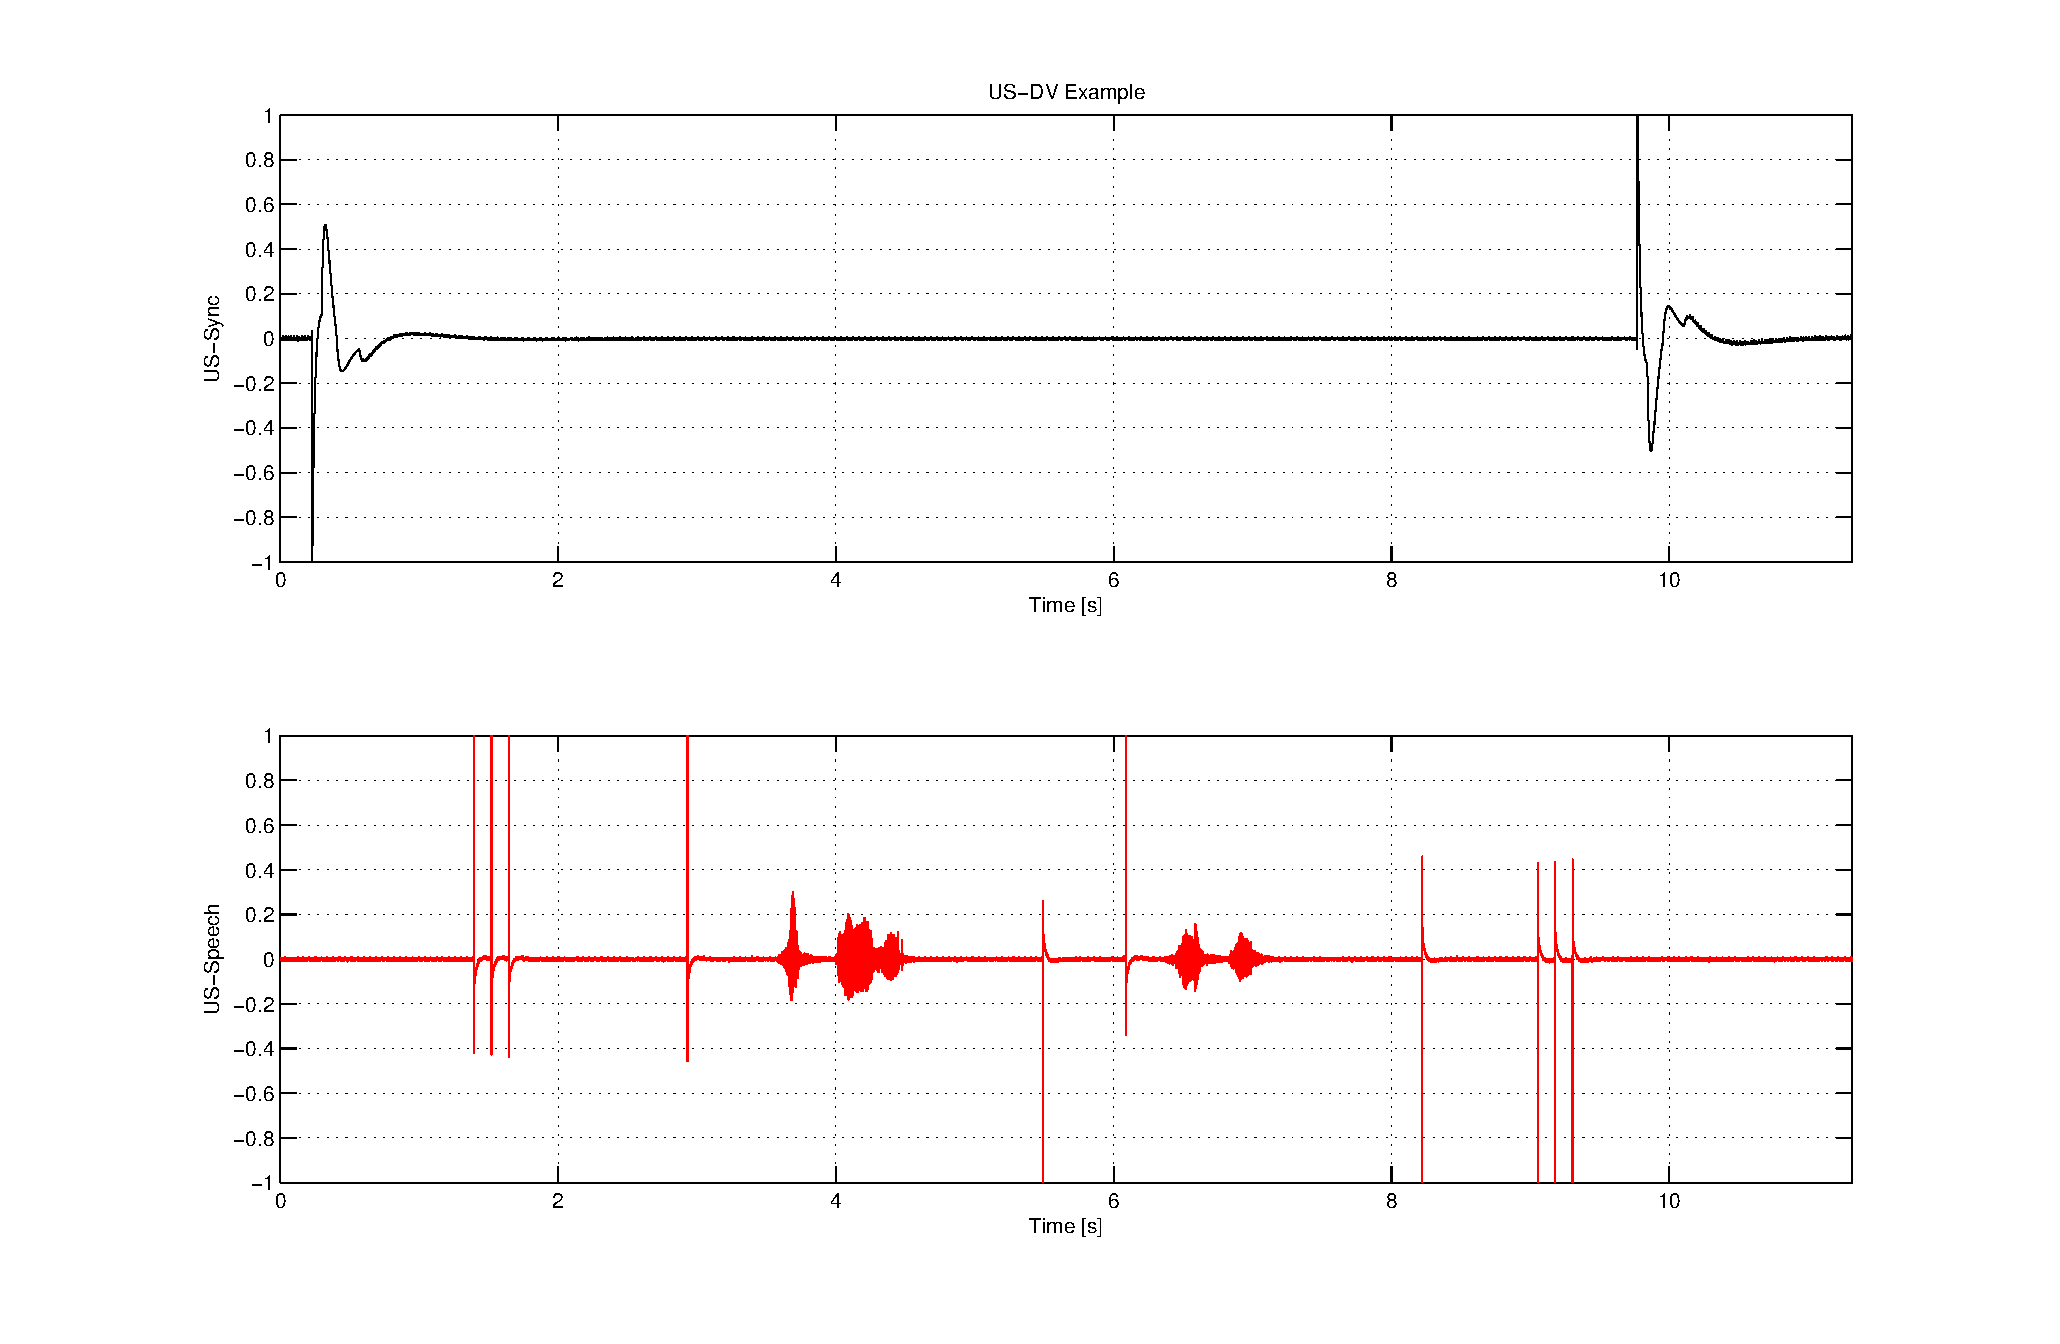
\epsfig{file=include/linguometer/images/usdv_example.eps,width=1.00\textwidth}
	\caption[US-DV Example]{\textbf{US-DV Example}: 
	(a) \wf{US-Sync} and (b) \wf{US-Speech} signals.}
	\label{fig:linguometer:architecture:sig:usdv}
\end{figure}
% ---------------------------------------------------------------------------- %

Figure~\ref{fig:linguometer:architecture:workflow} shows a symbolic
representation of the data \wf{US-DV} stream; 
a total of ten time-labels are used to highlight the time instants that play a
crucial role int the synchronization mechanism. 
Eight out of the ten labels are linked with a particular
synchronization/segmentation signal.

On the other hand, Figure~\ref{fig:linguometer:architecture:sig:usdv} shows a 
real example of the \wf{US-DV} track albeit the signals strictly 
resembles what already
discussed in Section~\ref{sec:linguometer:architecture:diagram} (a batch of two words
is used) (?on the other hand/albeit?).
The upper plot refers to the left audio channel and shows the \wf{US-Sync}
signal. Two peaks are visible: the first one reaches the negative saturation
value (\tstart{AG}) while the latter one reaches the positive saturation value 
(\tstop{AG}).
In the lower plot the \wf{US-Speech} signal is shown. This signal contains two
  main components: the speech signal itself and the segmentation signals.
A total of ten peaks are shown.
The first three peaks reach the positive saturation value and the distance
between each other is constant. 
Those peaks constitute the \emph{word batch start} signal.
Similarly, at the very end of the track, the \emph{word batch stop} signal is
shown (the cluster of three peaks that reach the negative saturation value).

The remaining four peaks constitute the \emph{word start/stop} segmentation
signals.
The first word\footnote{First word: /mattone/, /brick/ in English.}
is delimited by the fourth and the fifth peak
(\tstarti{WD}{0}, and \tstopi{WD}{0})
while the latter one\footnote{Second word: /goffo/, /clumsy/ in English.}
is delimited by the sixth and the seventh peak 
(\tstarti{WD}{1}, and \tstopi{WD}{1}).
As already discussed, the segmentation signals are generated by the
\emph{lmwords} stimuli presentation program, here described in detail.
% ---------------------------------------------------------------------------- %
\subsection{Stimuli presentation program: \emph{lmwords}}
\label{sec:linguometer:technical:lmwords}
% ---------------------------------------------------------------------------- %
Although the stimuli presentation program is very simple and does not enclose
any distinctive feature, the author believes that its functionality has to be
discussed to better explain how the segmentation signals are generated. 
Furthermore, from a less-technical perspective, the reader may find interesting
to know how the stimuli are presented to the recorded subjects.

\emph{lmwords} is written in C++ on and relies on the \emph{SDL} library (Simple
DirectMedia Layer)\footnote{libsdl v.1.2.11-r2, http://www.libsdl.org/.} 
for stimuli presentation and segmentation signal generation.
Providing a straightforward interface and a comprehensive set of plug-ins, 
SDL appeared as the best choice.
\emph{lmwords} instantiates a full-screen black window in which the stimuli are
rendered using the \emph{sdl-ttf} library (SDL TrueType Fonts
lib.)\footnote{sdl-ttf v.2.0.8 http://www.libsdl.org/projects/SDL\_ttf/.}.
The stimuli-presentation window is shown on a secondary monitor managed by
\sig{PC0}. The segmentation signals have been created ad-hoc using a
\emph{LMTools} library that provides the methods to handle PCM streams and their
encoding via an FFMPEG interface\footnote{ffmpeg v.0.4.9, http://ffmpeg.org/.}.
% ---------------------------------------------------------------------------- %
\begin{figure}
	\centering
	\subfigure[\label{fig:linguometer:architecture:sig:lmwords2:1}]
	{\includegraphics[width=0.25\textwidth]{include/linguometer/images/lmwords_1.tps}}
	\hspace{0.05\textwidth}
	\subfigure[\label{fig:linguometer:architecture:sig:lmwords2:2}]
	{\includegraphics[width=0.25\textwidth]{include/linguometer/images/lmwords_2.tps}}
	\hspace{0.05\textwidth}
	\subfigure[\label{fig:linguometer:architecture:sig:lmwords2:3}]
	{\includegraphics[width=0.25\textwidth]{include/linguometer/images/lmwords_3.tps}}

	\subfigure[\label{fig:linguometer:architecture:sig:lmwords2:4}]
	{\includegraphics[width=0.25\textwidth]{include/linguometer/images/lmwords_4.tps}}
	\hspace{0.05\textwidth}
	\subfigure[\label{fig:linguometer:architecture:sig:lmwords2:5}]
	{\includegraphics[width=0.25\textwidth]{include/linguometer/images/lmwords_5.tps}}
	\hspace{0.05\textwidth}
	\subfigure[\label{fig:linguometer:architecture:sig:lmwords2:6}]
	{\includegraphics[width=0.25\textwidth]{include/linguometer/images/lmwords_6.tps}}
	
	\caption[Stimuli-presentation program states]{\textbf{Stimuli-presentation 
	program states}: \emph{lmwords} passes through four distinct states: (a)
	\emph{pause}, (b) \emph{ready}, (c,d) \emph{word presentation} and
	(e) \emph{done}. The last panel (f) shows how the stimuli are presented on 
	the LCD screen used during the recording sessions.
	During each state-transition, the screen remains black for half a second.
	Furthermore, the subjects are aware of meaning of each state. 
	In fact, the subjects can freely talk to the experimenters until the program
	enters in the ``pause'' state and after the program enters the ``end''
	state.}
	\label{fig:linguometer:architecture:sig:lmwords}
\end{figure}
% ---------------------------------------------------------------------------- %

Those signals are loaded and played by \emph{lmwords} using the \emph{sdl-mixer}
library\footnote{sdl-mixer v.1.2.7,
http://www.libsdl.org/projects/SDL\_mixer/.}.

The \emph{lmwords} program has four main states: \emph{pause}, \emph{ready},
\emph{word presentation} and \emph{done}.
After it has been launched, \emph{lmwords} loads a batch of stimuli and mixes it
randomly, although the seed that is used to generate the normal distribution has
been kept fixed during the linguometer experiments.
The first state entered by the program is ``pause''. By pressing a key on
the \sig{PC0} keyboard, the experimenter generates the \emph{word batch start}
segmentation signal and the program enters the ``ready'' state, waiting for
user input.

% ---------------------------------------------------------------------------- %
\begin{figure}
	\centering
	\subfigure[\label{fig:linguometer:architecture:sig:lmwords:1}]
	{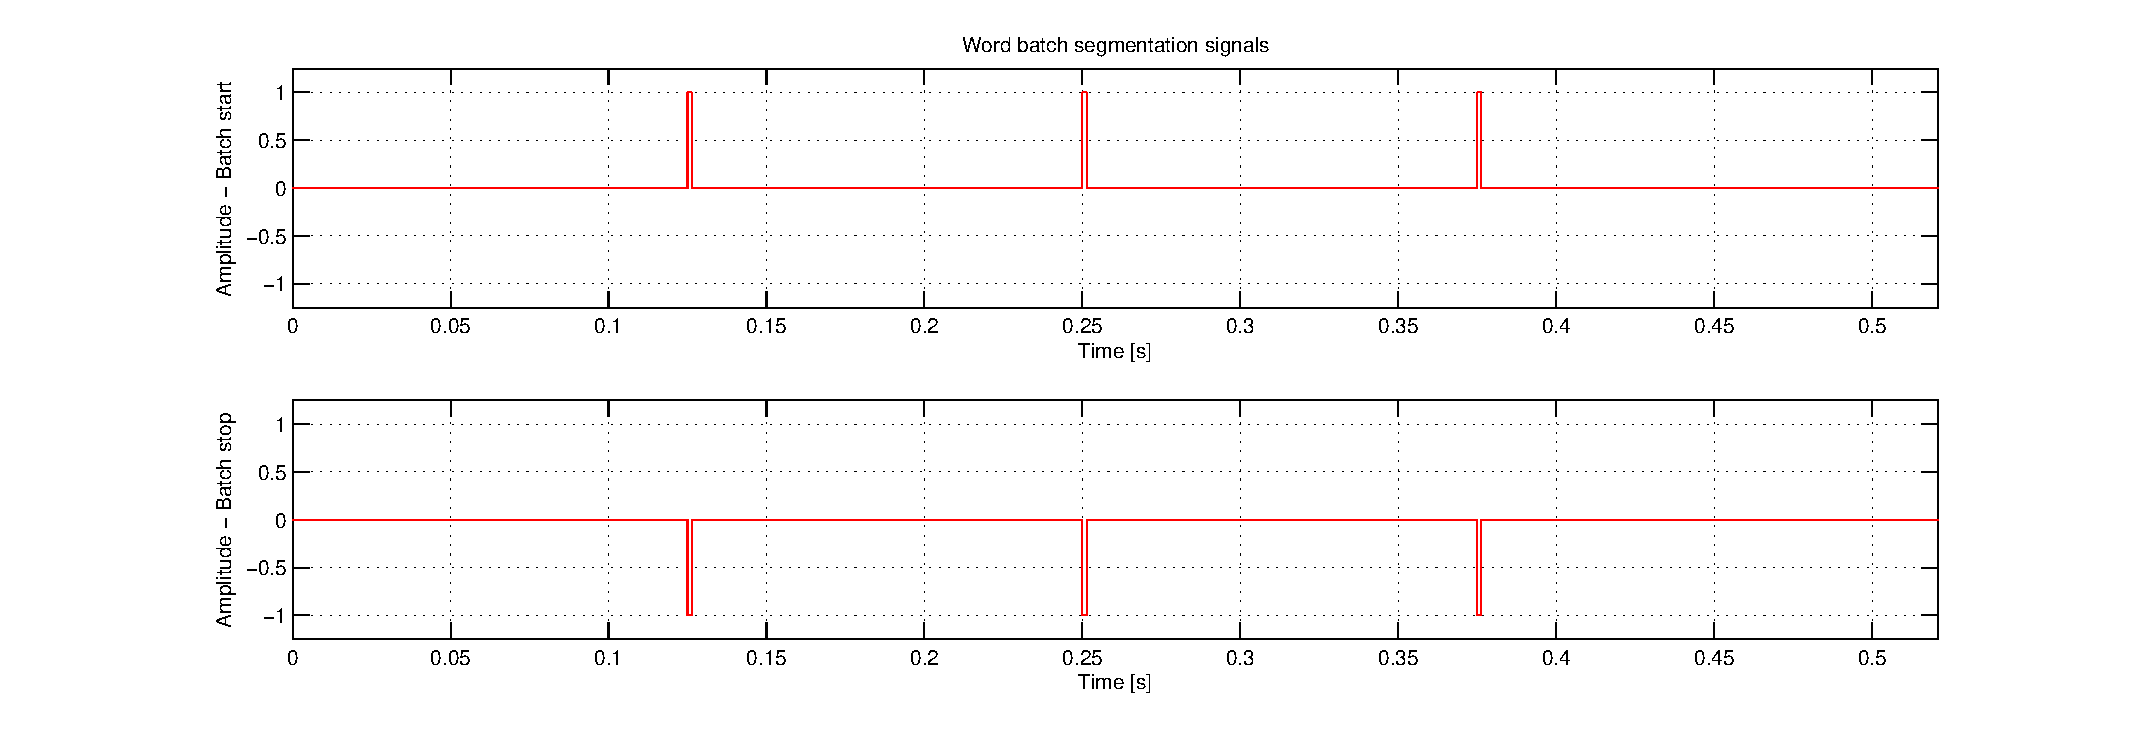
\includegraphics[width=\textwidth]{include/linguometer/images/seg_batch.eps}}
	
	\subfigure[\label{fig:linguometer:architecture:sig:lmwords:2}]
	{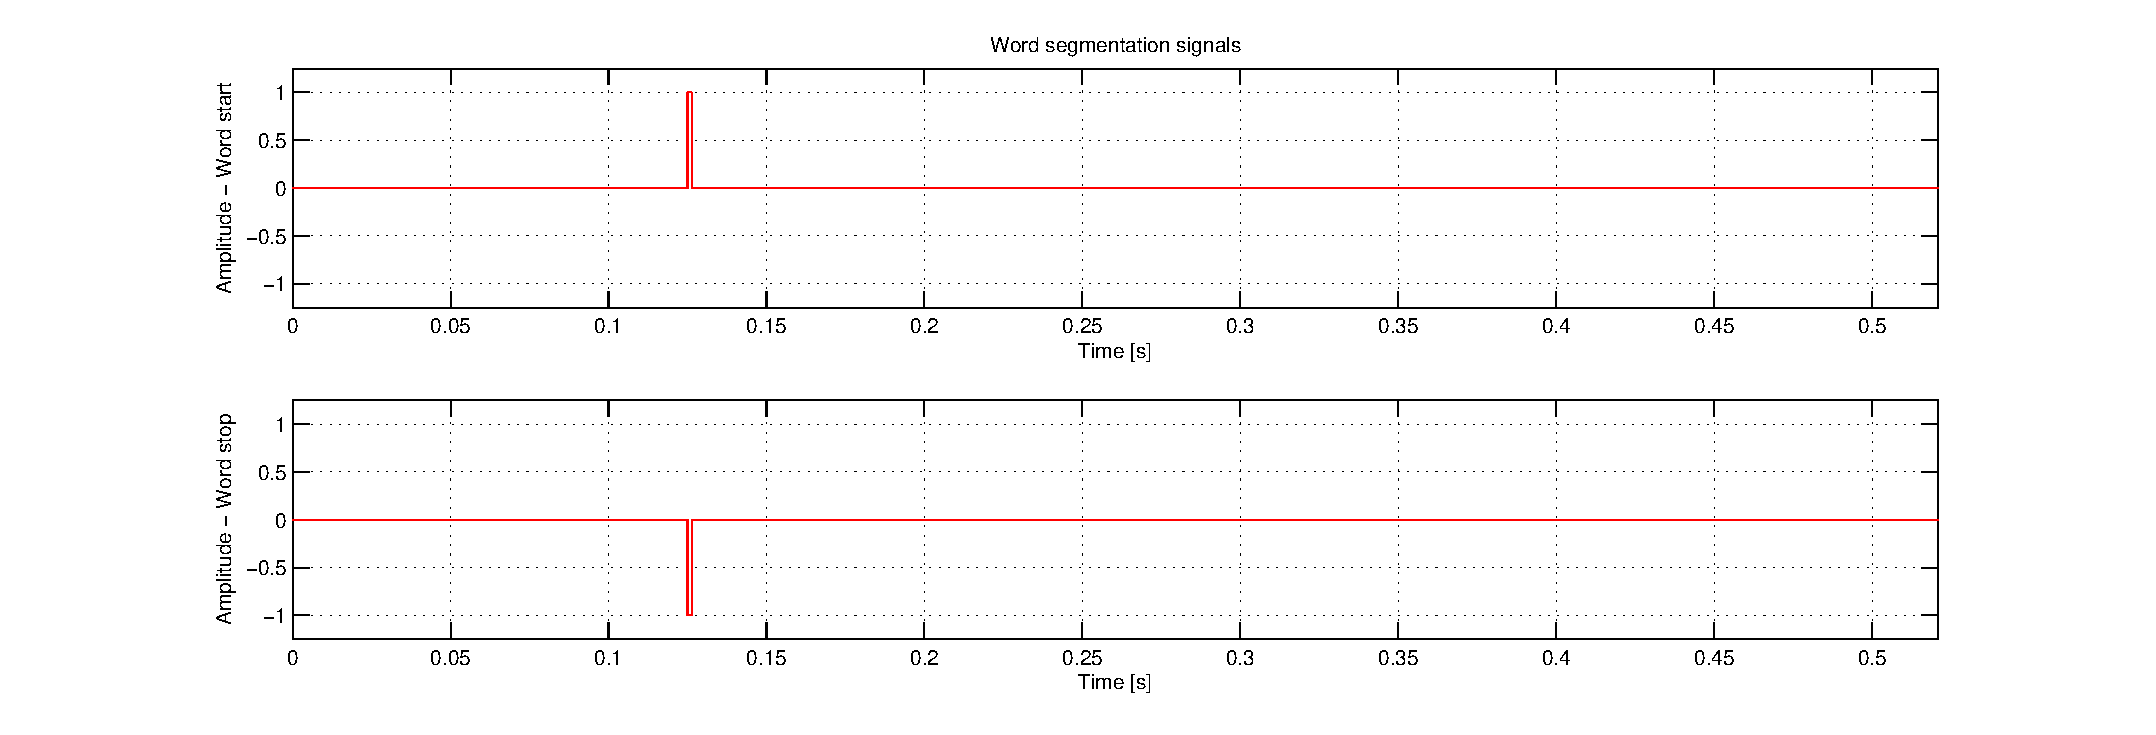
\includegraphics[width=\textwidth]{include/linguometer/images/seg_word.eps}}
	
	\caption[Segmentation signals]{\textbf{Segmentation signals}:
	the right channel component of the segmentation signals is shown (the left 
	channel has zero amplitude):
	(a) \emph{word batch start/stop} and (b) \emph{word start/stop}.
	The duration of the signals is 520 ms, while the duration of
	the peaks is 1.33 ms (64 samples). The first peak appears after 124 ms from
	the beginning of the tracks.
	In (a) the delay between two contiguous peaks is set to 124 ms. 
	Note: the amplitude axis interval is set to $[-1.50, 1.50]$ although
	the negative and positive saturation values are set to $-1.00$ and $1.00$
	respectively.
	The signals are stored in a Microsoft WAV container (PMC 16bit, 48kHz).
	}
	\label{fig:linguometer:architecture:sig:segmentation}
\end{figure}
% ---------------------------------------------------------------------------- %

Another key press causes \emph{lmwords} to enter the ``word presentation''
state: the \emph{word start} signal is generated and the first word is 
rendered on the screen.
The program remains into the last state until the experimenter has decided if
the presented stimuli have been pronounced correctly by the subject.
In fact, the experimenter, by pressing a key, can mark the word as ``correctly
pronounced'' or ``mispronounced''. 
In both cases, \emph{lmwords} generates the \emph{word stop} signal and 
moves to the next stimulus.
In the case that the word is mispronounced by the subject, \emph{lmwords} queues
the stimulus so it will be presented at the end of the batch.
Once the whole set of stimuli has been presented and the whole pronounced words
have been marked as ``correctly pronounced'' by the experimenter,
\emph{lmwords} enters generates the \emph{word batch stop} signal and enters 
the ``done'' state.
Figure~\ref{fig:linguometer:architecture:sig:lmwords} shows the four
states entered by \emph{lmwords} while 
in Figure~\ref{fig:linguometer:architecture:sig:segmentation} the segmentation
signals are shown.
% ---------------------------------------------------------------------------- %
\subsection{Acquisition card and audio mixer delay}
\label{sec:linguometer:technical:delay}
% ---------------------------------------------------------------------------- %
The time delays that affects both the acquisition card and the 
audio mixer have been measured.
As already discussed in this Section, those two devices are the core of the
articulographic/ultrasonograpic data hardware synchronization mechanism.
Although the values of the measured delays appear qualitatively small, knowing 
them is surely useful for what regards the post-processing alignment task.
% ---------------------------------------------------------------------------- %
\begin{figure}
	\centering
	\subfigure[\label{fig:linguometer:architecture:sig:delay:7}]
	{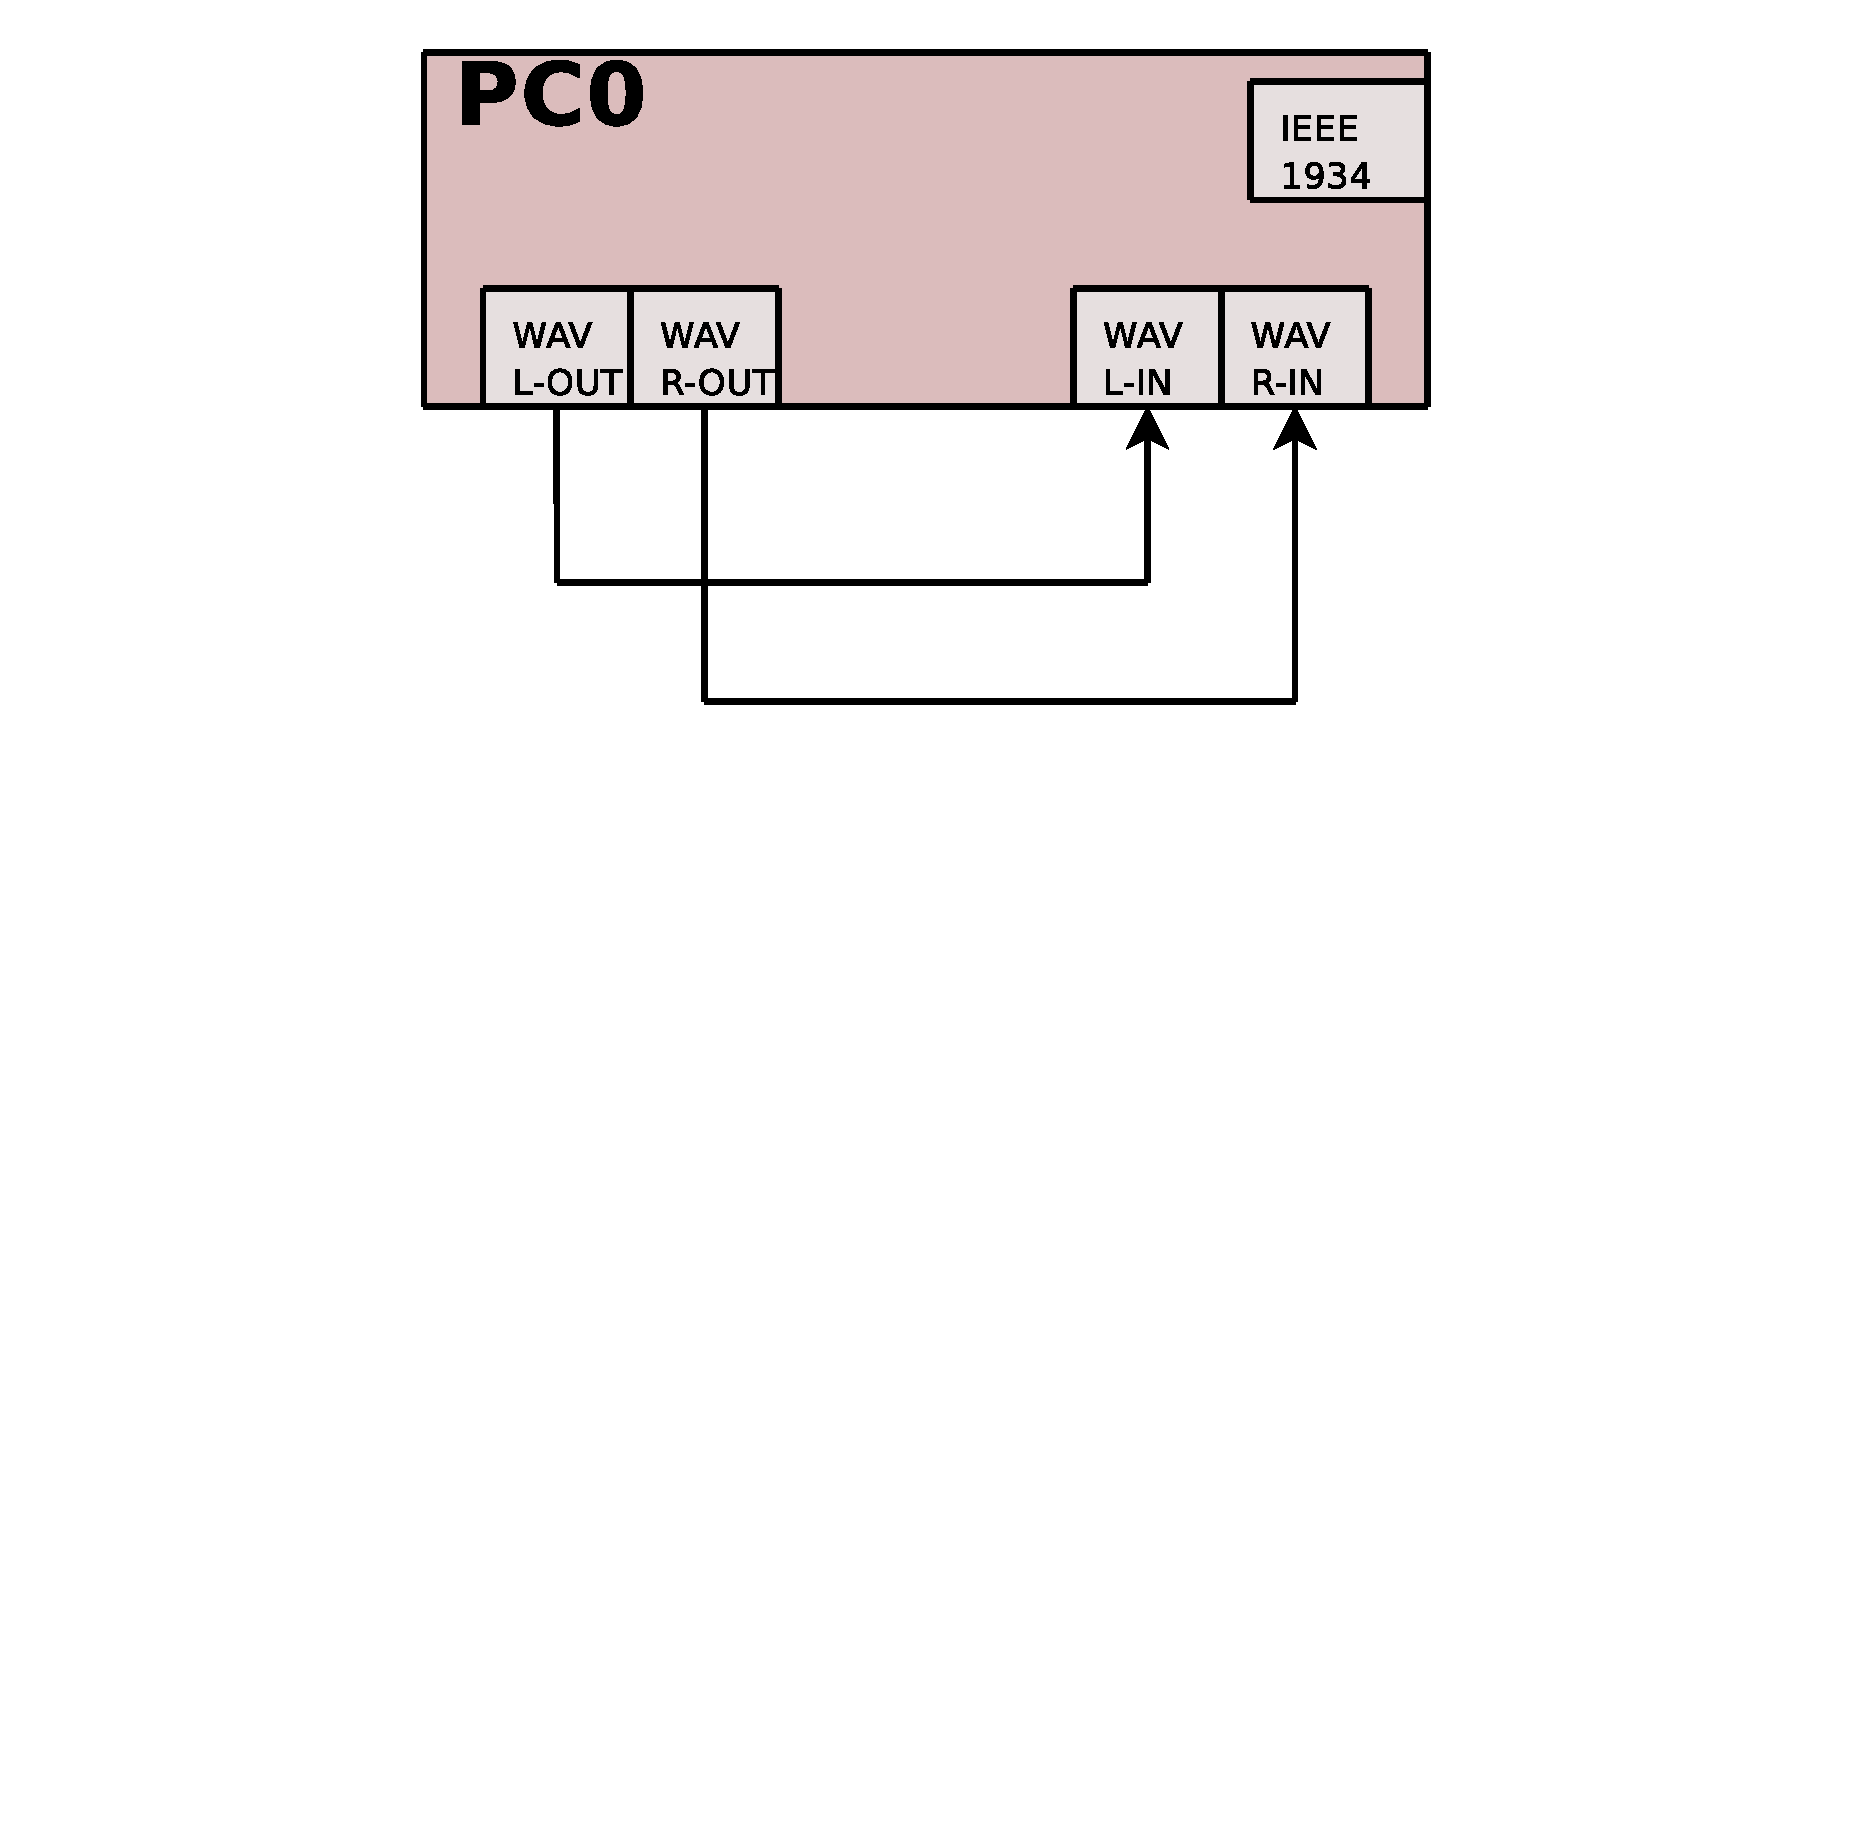
\includegraphics[width=0.32\textwidth]{include/linguometer/images/delay_schemaT.eps}}
	\subfigure[\label{fig:linguometer:architecture:sig:delay:8}]
	{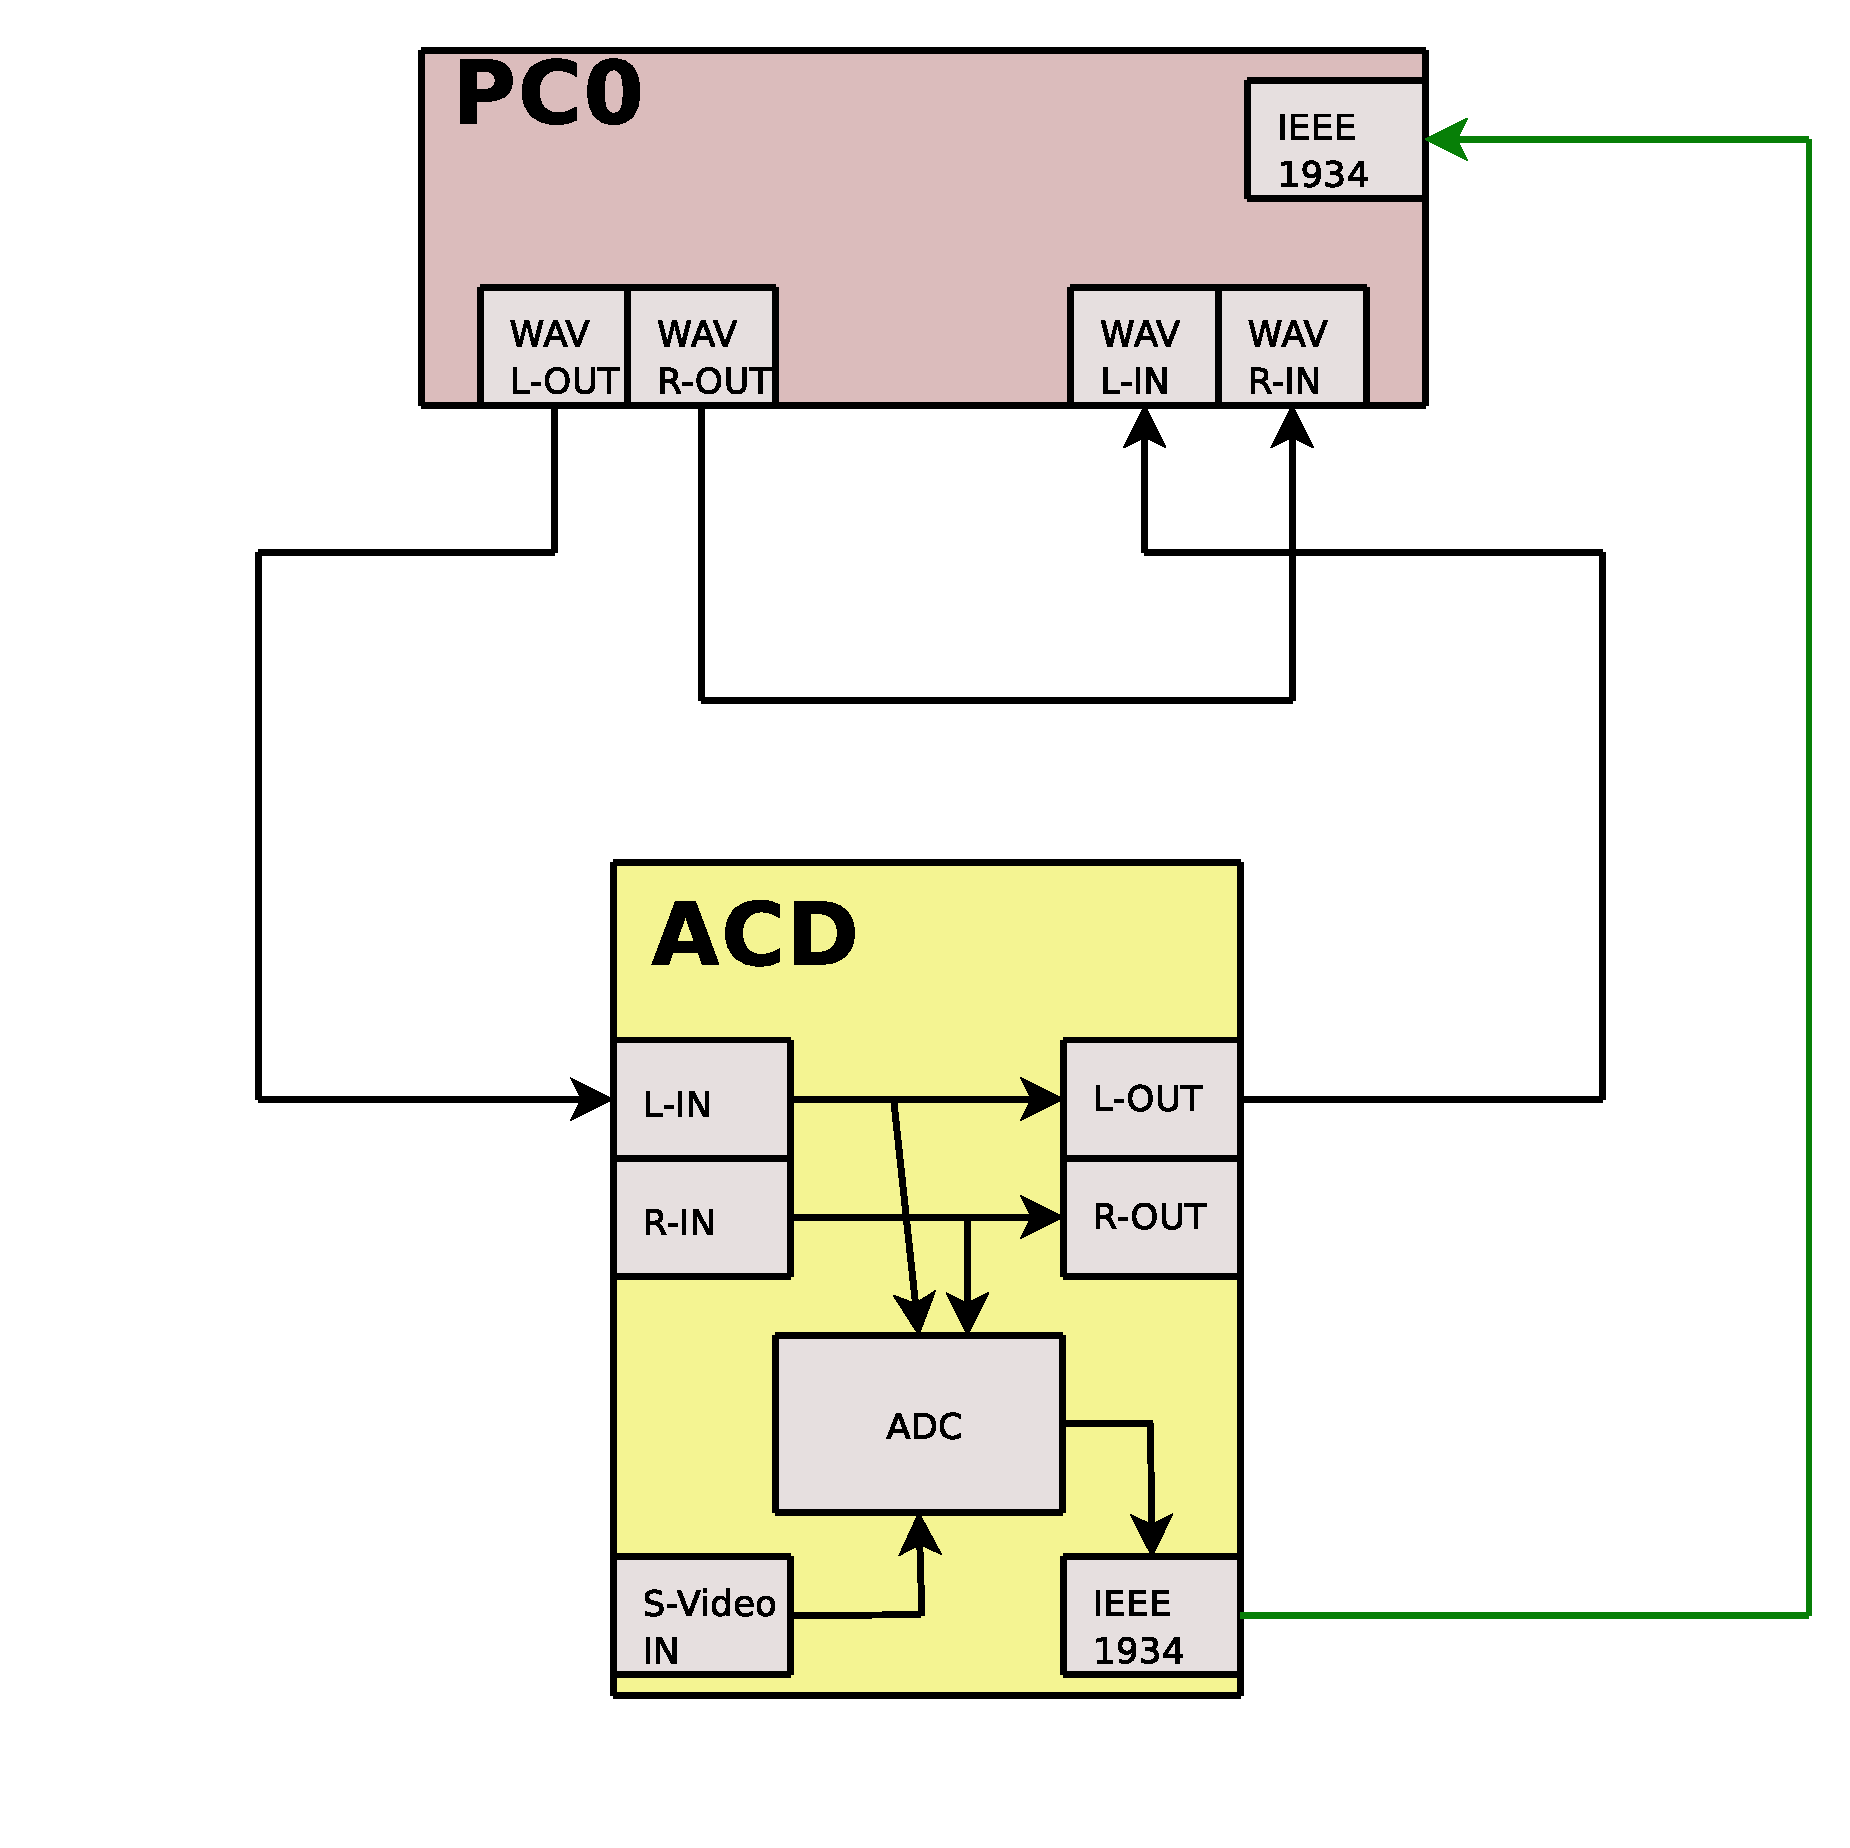
\includegraphics[width=0.32\textwidth]{include/linguometer/images/delay_schemaL.eps}}
	\subfigure[\label{fig:linguometer:architecture:sig:delay:9}]
	{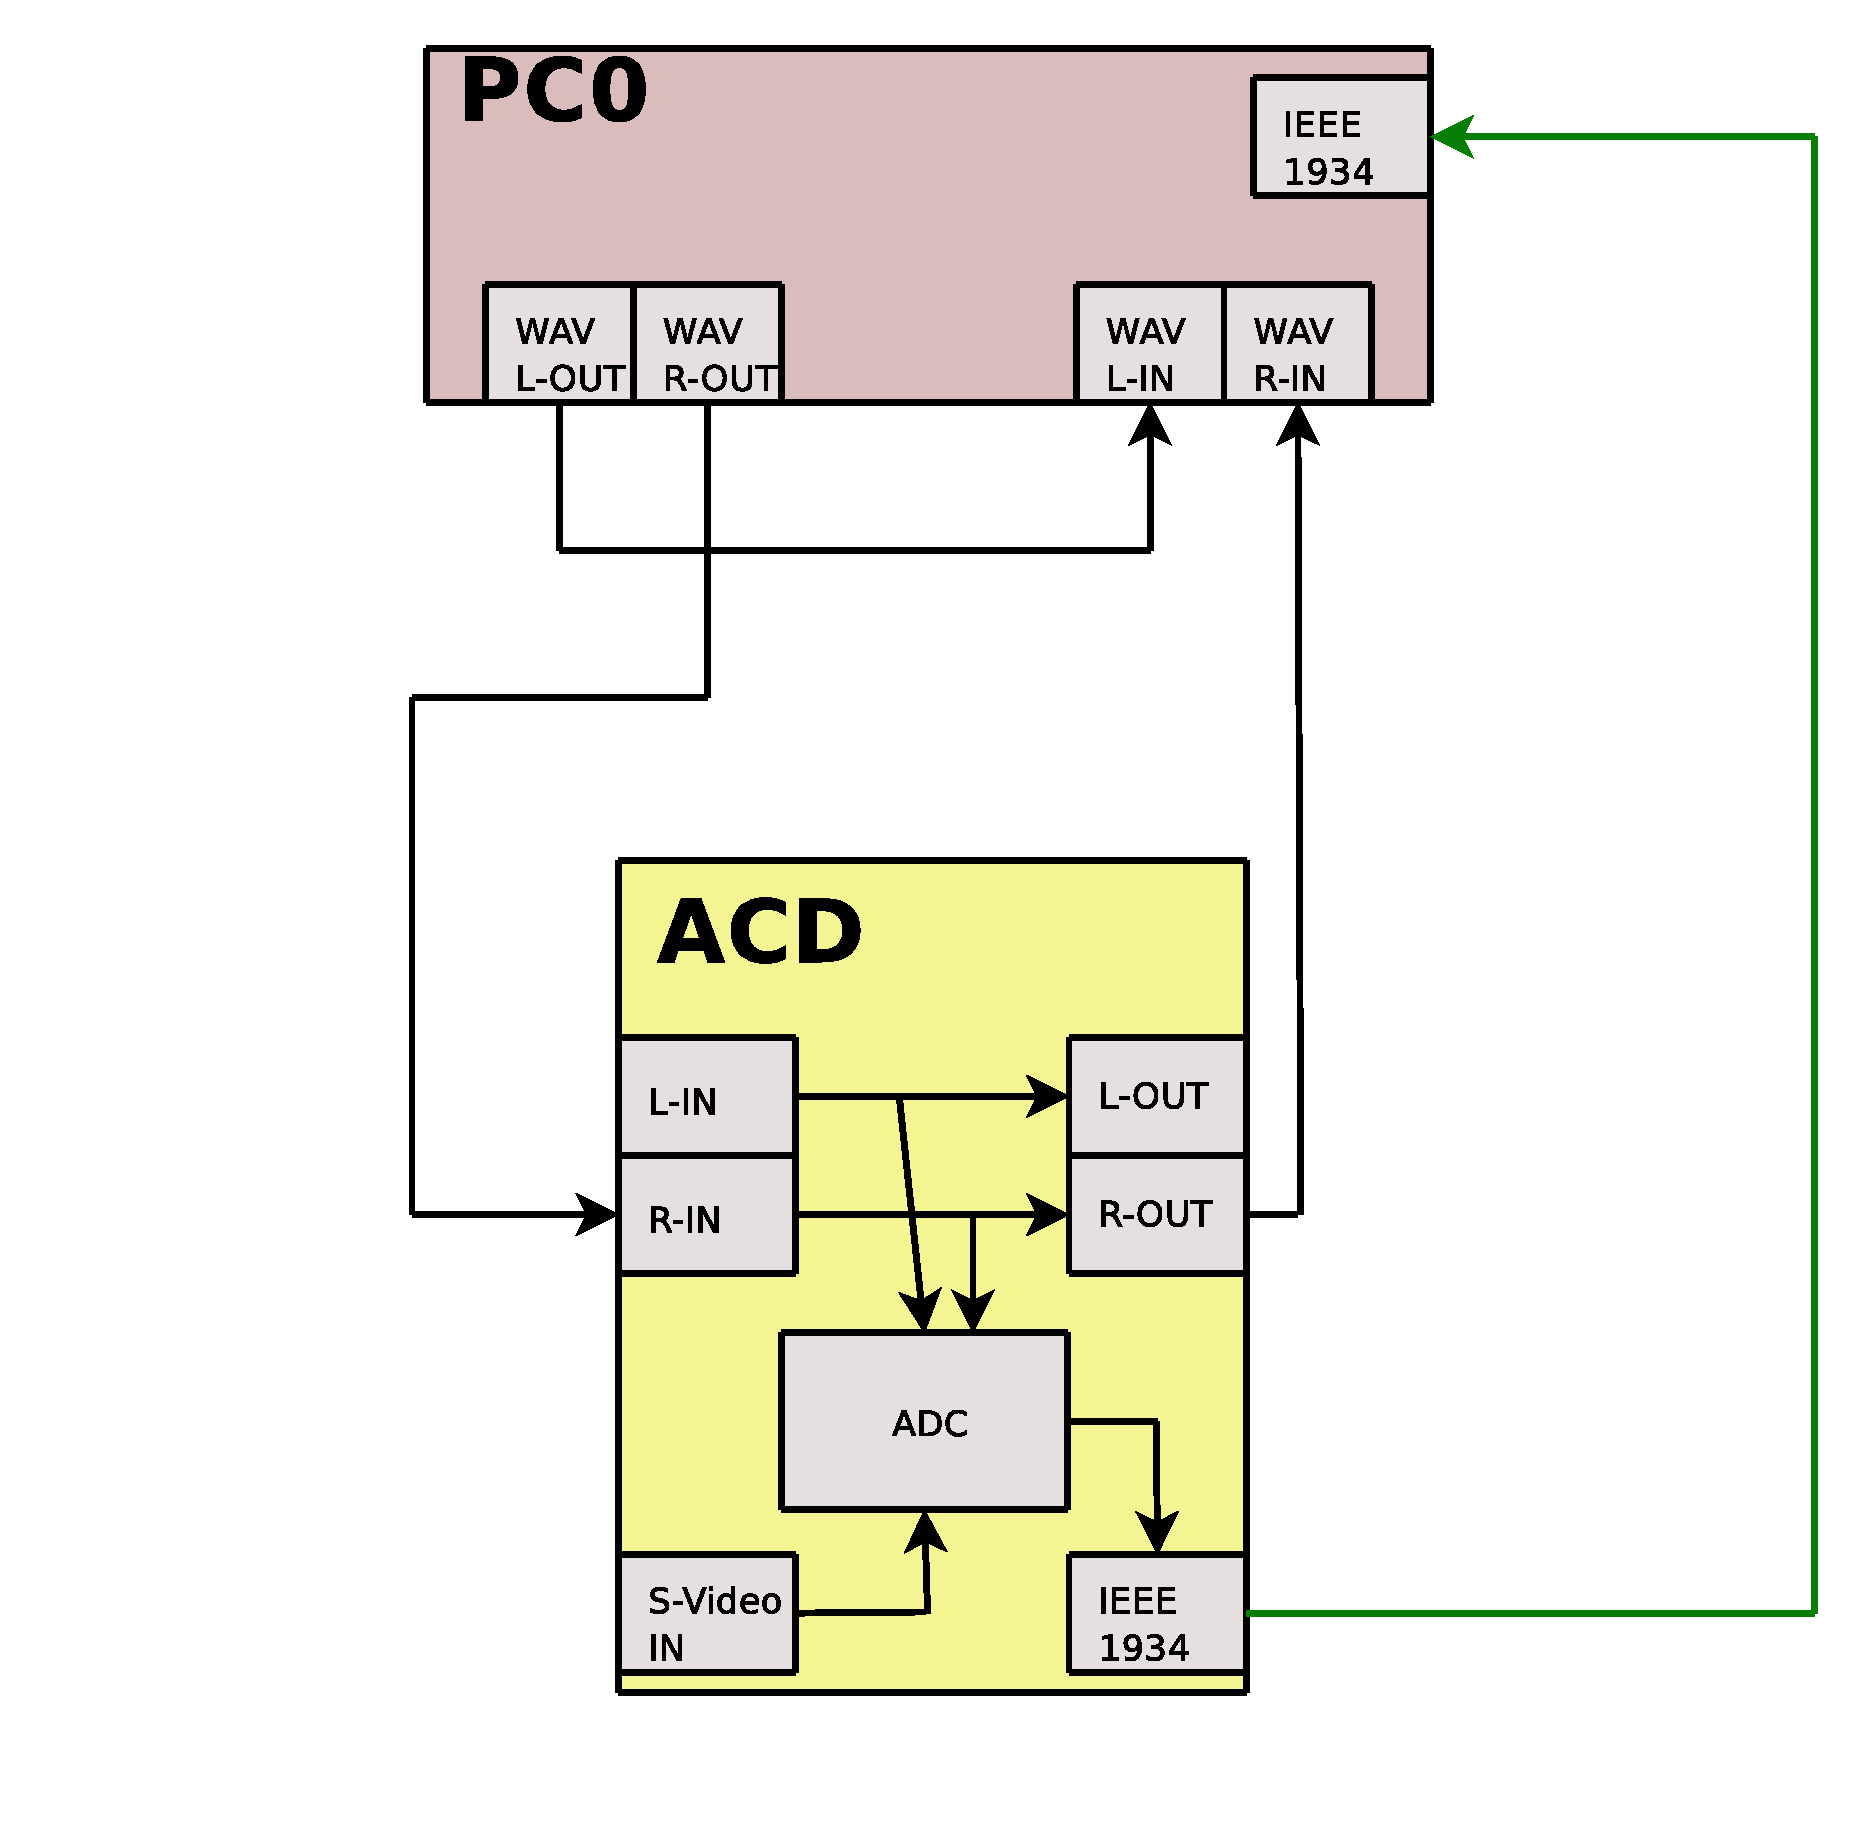
\includegraphics[width=0.32\textwidth]{include/linguometer/images/delay_schemaR.eps}}

	\subfigure[\label{fig:linguometer:architecture:sig:delay:1}]
	{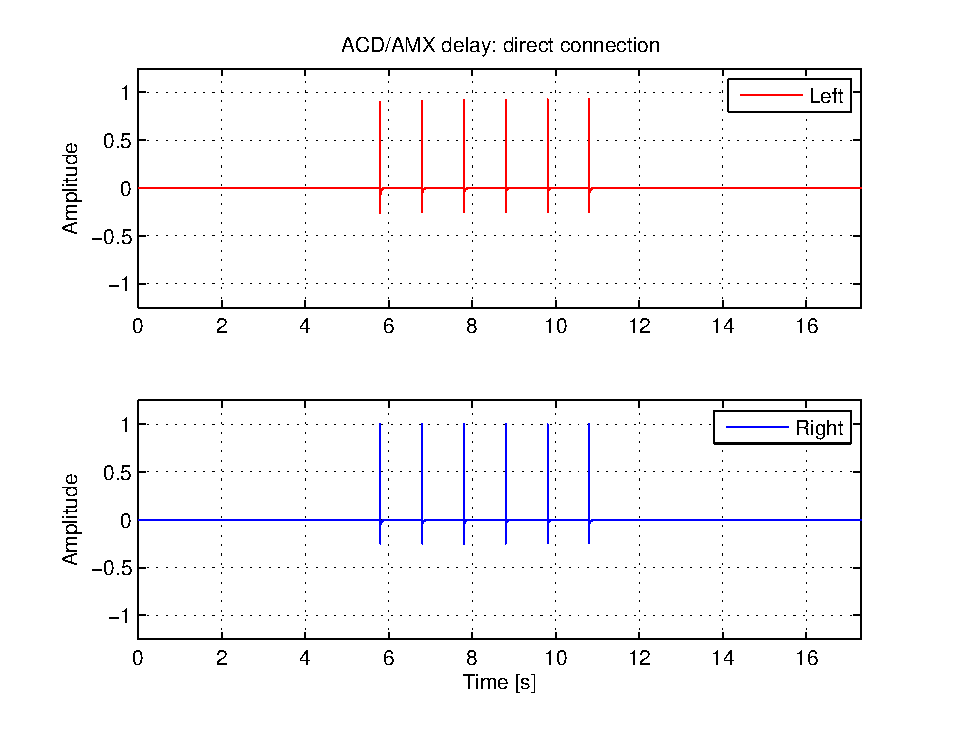
\includegraphics[width=0.32\textwidth]{include/linguometer/images/delay_fullT.eps}}
	\subfigure[\label{fig:linguometer:architecture:sig:delay:2}]
	{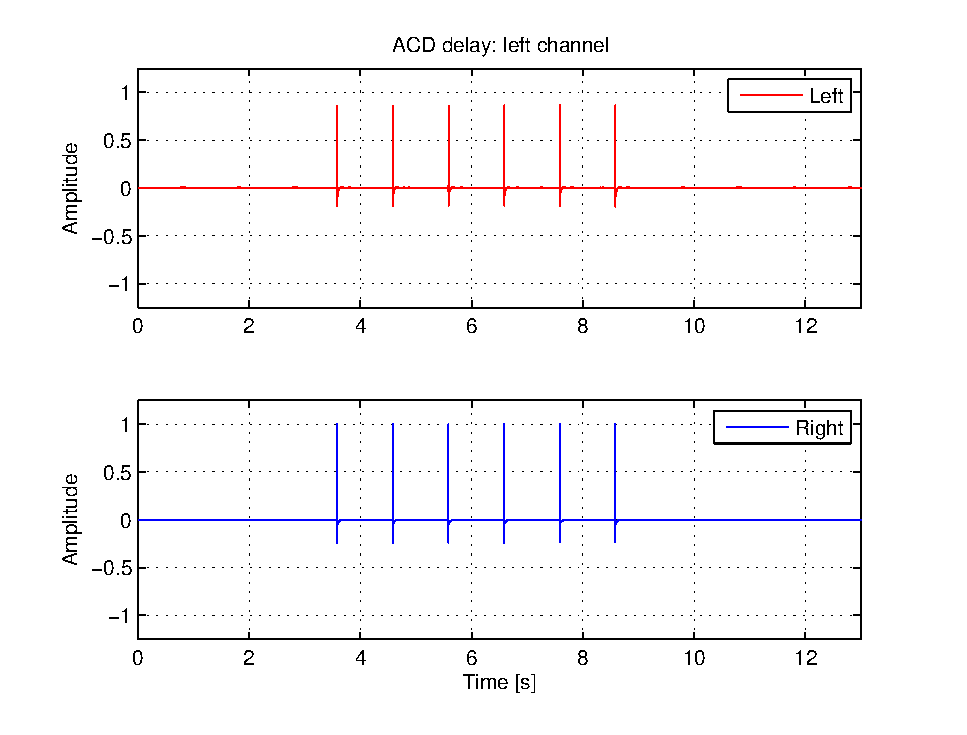
\includegraphics[width=0.32\textwidth]{include/linguometer/images/delay_fullL.eps}}
	\subfigure[\label{fig:linguometer:architecture:sig:delay:3}]
	{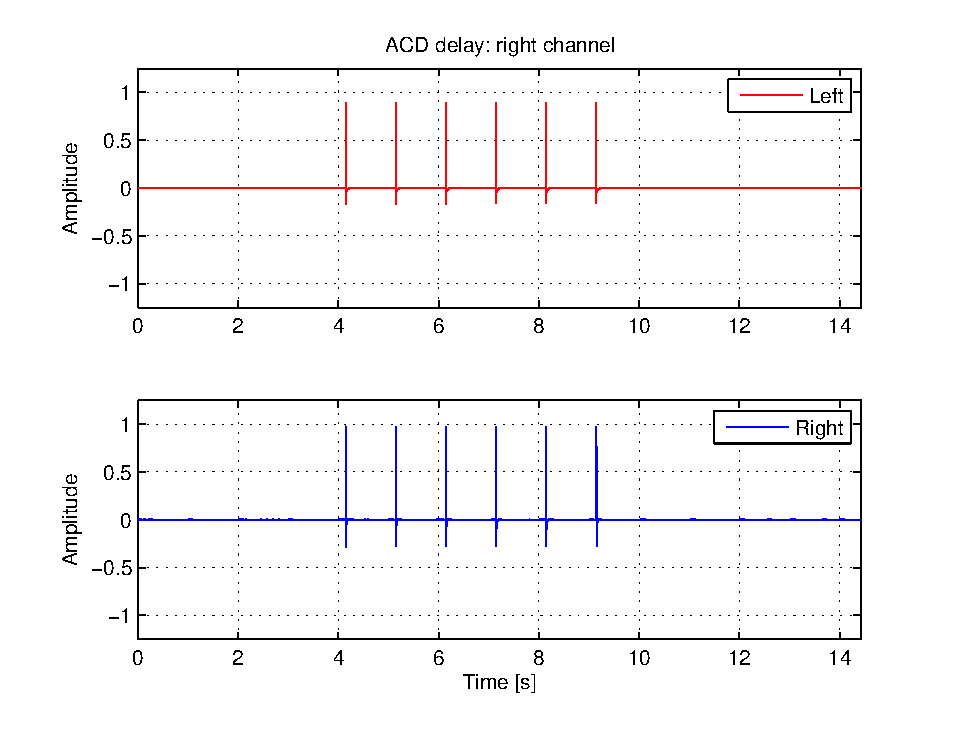
\includegraphics[width=0.32\textwidth]{include/linguometer/images/delay_fullR.eps}}
	
	\subfigure[\label{fig:linguometer:architecture:sig:delay:4}]
	{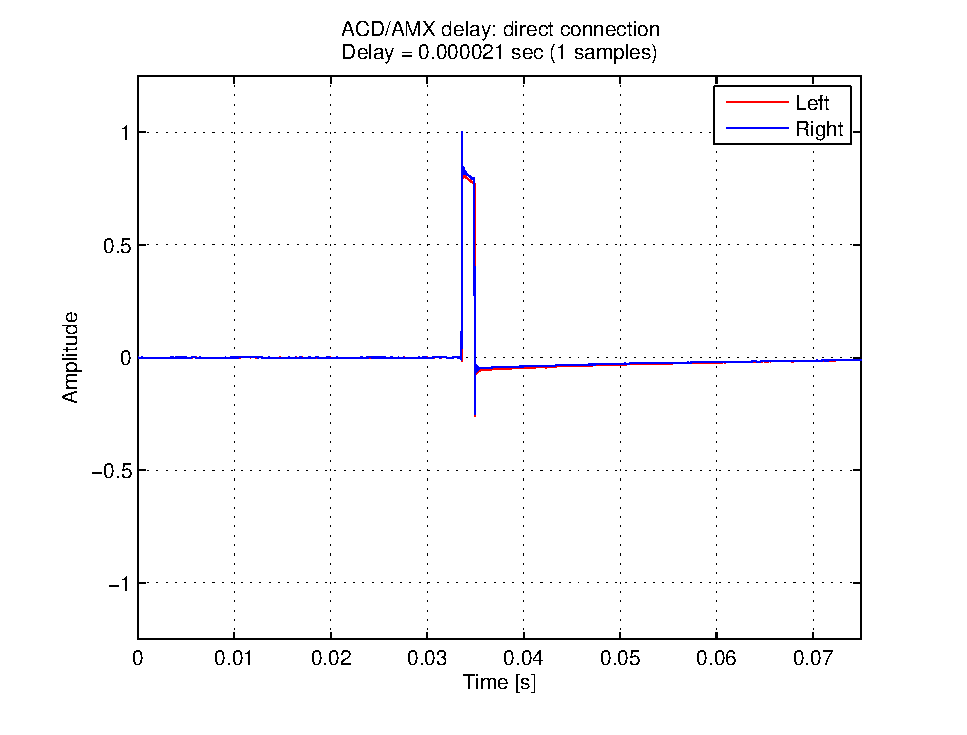
\includegraphics[width=0.32\textwidth]{include/linguometer/images/delay_zoomT.eps}}
	\subfigure[\label{fig:linguometer:architecture:sig:delay:5}]
	{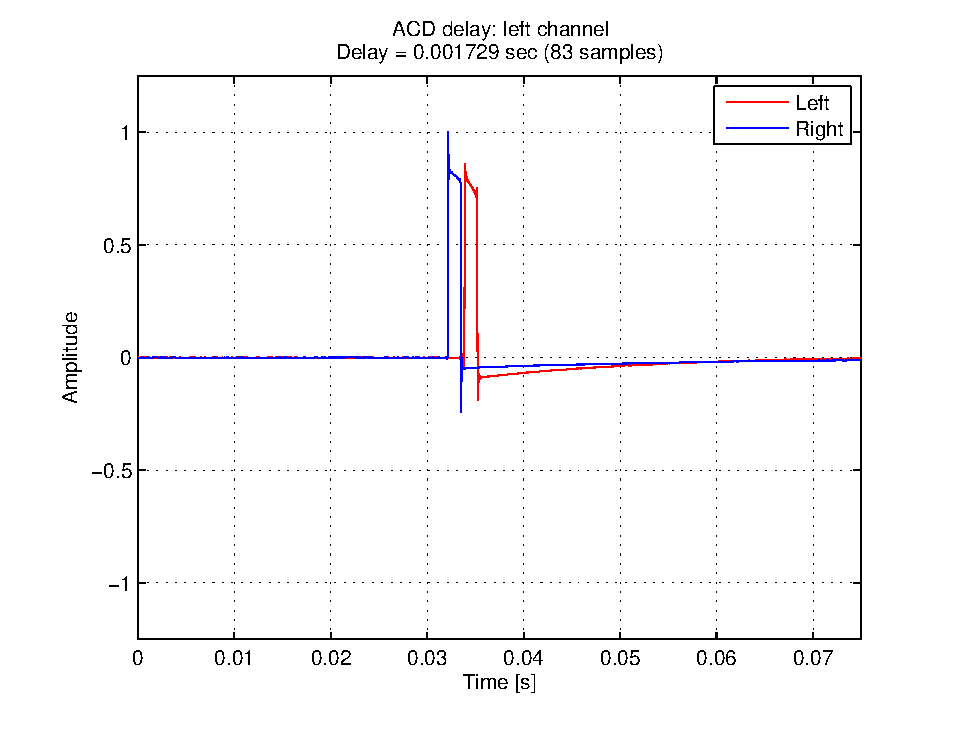
\includegraphics[width=0.32\textwidth]{include/linguometer/images/delay_zoomL.eps}}
	\subfigure[\label{fig:linguometer:architecture:sig:delay:6}]
	{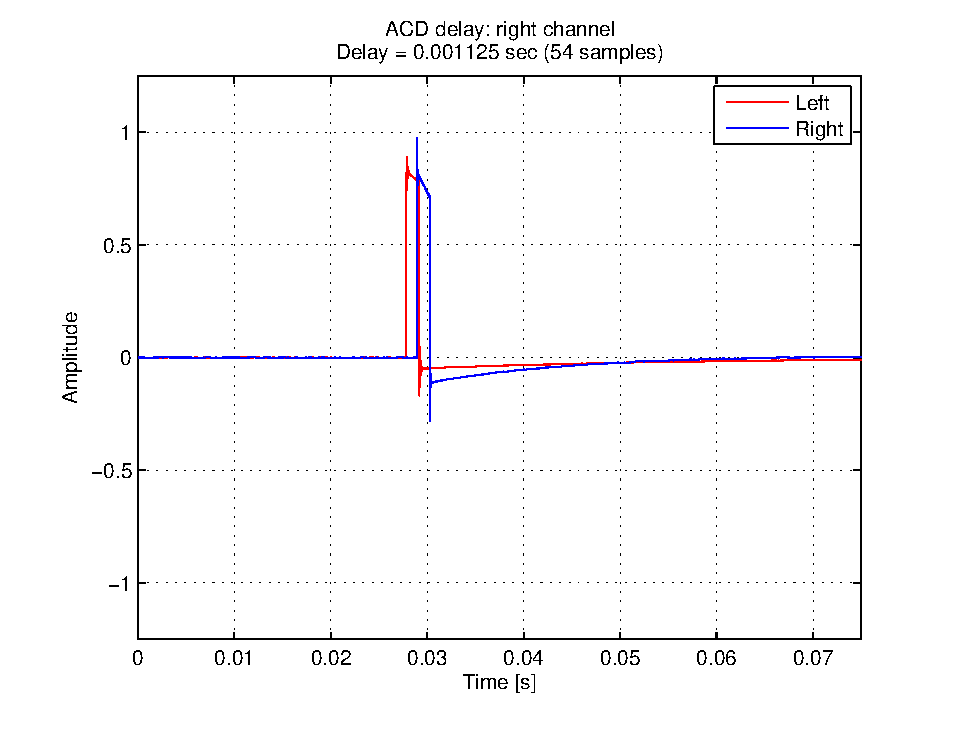
\includegraphics[width=0.32\textwidth]{include/linguometer/images/delay_zoomR.eps}}
	
	\caption[Acquisition card delay]{\textbf{Acquisition card delay}:
	(a) direct connection (reference test);
	(b) left channel trough the delayed device;
	(c) right channel trough the delayed device.
	(d, e, f) Test signals as they are acquired by \sig{PC0}.
	(g, h, i) Firts peak of the acquired signals.
	The plots refer to the first trial.
	}
	\label{fig:linguometer:architecture:sig:delay}
\end{figure}
% ---------------------------------------------------------------------------- %

The author measured the delays that affect the \sig{AMX} mixer
\sig{Line1 L-IN}/\sig{Mixer L-OUT} and the
\sig{Line1 R-IN}/\sig{Mixer R-OUT} connections.
Furthermore, the  \sig{ACD} acquisition card
\sig{L-IN}/\sig{L-OUT} and
\sig{R-IN}/\sig{R-OUT} delays have been measured.

In order to measure the delays, the setup control computer \sig{PC0} has been 
used.
A stereo audio signal with a total of six peaks has been built, 
following the same procedure used for the \emph{lmwords} segmentation signals
(PCM 16 bit, 48kHz).
The main idea behind the delay test is trivial. The test signal is made up by
two identical channels, each one with six peaks.
The digital signal is converted in its analog form by \sig{PC1}, simply using
its sound card (line level outputs).
One out of the two channels is routed trough the delay-affected device and then
back to \sig{PC1}, using the sound card line level inputs.
The remaining channel, used as reference, is routed directly
from the line level output connector to the line level input connector.
Being the original channels perfectly synchronized, if the measured device
introduce some kind of time shift in the signal, it should be detectable by the
means of cross-correlation.
Figure~\ref{fig:linguometer:architecture:sig:delay} shows the building blocks
and the resulting signals obtained measuring the acquisition card delay.

A total of five different tests have been executed, three times each.
In the first case, the test signal is routed directly from the line level output
to the line level input connector, as shown in
Figure~\ref{fig:linguometer:architecture:sig:delay:7}.
In the second and third cases,
Figures~\ref{fig:linguometer:architecture:sig:delay:8} and
and~\ref{fig:linguometer:architecture:sig:delay:9},
the \sig{ACD} \sig{L-IN}/\sig{L-OUT} and
the \sig{R-IN}/\sig{R-OUT} delays have been measured routing one audio channel
at the time (\sig{WAV L-OUT} and \sig{WAV R-OUT}) trough the delay-affected
device (in this case, \sig{ACD}).
In the latest two cases, the \sig{AMX} \sig{Line1 L-IN}/\sig{Mixer L-OUT} and 
\sig{Line1 R-IN}/\sig{Mixer R-OUT} delays have been measured, following the same
procedure used to measure the \sig{ACD} delays.
%The left and the right channels of the test signal are identical. 
%In other words the peak appear at the same time in both the channels.
Figures~\ref{fig:linguometer:architecture:sig:delay:1}, 
\ref{fig:linguometer:architecture:sig:delay:2} and
\ref{fig:linguometer:architecture:sig:delay:3} show the test signal 
as recorded by the \sig{PC0} \sig{WAV L-IN}/\sig{WAV R-IN} line level input.\\
Figures~\ref{fig:linguometer:architecture:sig:delay:4}, 
\ref{fig:linguometer:architecture:sig:delay:5} and
\ref{fig:linguometer:architecture:sig:delay:6} show the
first peak of the recorded test signal.
\begin{table}[ht!]
  \begin{center}
  \begin{scriptsize}
	\begin{tabular}{|c|c|cc|cc|}
	  \hline
	   & \textbf{Direct} & \textbf{ACD L.} & \textbf{ACD R.} & \textbf{AMX L.} & \textbf{AMX R.}\\
	  \hline
	  \textbf{Trial 1} & 1 & 83 & 54 & 22 & 24\\
	  \textbf{Trial 2} & 1 & 82 & 52 & 22 & 22\\
	  \textbf{Trial 3} & 2 & 83 & 53 & 25 & 23\\
	  \hline
	  \textbf{AVG} & 1.33 & 82.67 & 53.00 & 23.00 & 23.00\\
	  \textbf{STD} & 0.58 & 0.58 & 1.00 & 1.73 & 1.00\\
	  \hline
	  \textbf{AVG} (ms) & 0.028 & 1.722 & 1.104 & 0.480 & 0.480\\
	  \textbf{STD} (ms) & 0.012 & 0.021 & 0.021 & 0.036 & 0.021\\
	  \hline
  \end{tabular}
  \end{scriptsize}
  \end{center}
	\caption[Acquisition card and mixer delays]{\textbf{Acquisition card and
	mixer delays}: the last two rows values are in milliseconds. Where not
	specified, values are in samples.}
 \label {tab:linguometer:architecture:sig:delay}
\end{table}


Table~\ref{tab:linguometer:architecture:sig:delay} shows the results of the
three trials. As expected, the direct connection test is not affected by a
significant delay. The delays affecting the right and the left acquisition card
channels are not constant, although they are constant in time. 
On the other hand, the delays affecting the audio mixer appear to be constant
both between the two channels and in time.
% ---------------------------------------------------------------------------- %
\subsection{Ultrasonographic transducer: interference compensation}
\label{sec:linguometer:technical:interference}
% ---------------------------------------------------------------------------- %
As explained in the previous chapter, recording simultaneously with the
articulograph and the ultrasound system means placing the ultrasonograpic 
transducer inside the EMA-Cube frame of reference
(Section~\ref{ch:linguometer:instrumentation:custom}).
In this context, the ultrasonograpic transducer could  
modify the physical properties of the electromagnetic field generated by the six
AG500 reference coils, thus altering the acquired amplitudes
(Section~\ref{sec:linguometer:instrumentation:ag}).
An appropriate compensation of the interference in required in order not to
invalidate the kinesthetic information calculated from the recorded amplitudes.
In this section, the compensation of the interference is discussed.

Being the subjects' head free to move during the investigations, the positions
of the sensors attached to the articulators does need to be normalized over head
movement (\emph{ibid}).
%When recording the kinesthetic information of the articulators, it is clear
%that the recorded data does need to be compensated for head movement. 
Therefore, the author decided to attach a total of three sensors to a pair of 
glasses wear by the subjects during the experiments.
The glasses used for the linguometer experiments, shown in 
Figure~\ref{fig:linguometer:technical:glasses}, are designed to
fit young kids, thus they tightly fit adult subjects.
Furthermore, they endow the nice property of being shaped like an ``hearth''.
This last property is actually crucial, since the concave
zones facilitate the task of taping the sensors used for head motion
compensation, allowing the author to place the sensors always in the same
position.
However, the distance between the sensors was measured immediately after taping
those to the reference glasses.

%allowed to easily tape a pair of sensors suitable for recording
%head motion (!bleah!).
In summary, three sensors have been attached to the reference
glasses. The acquired information has been then used to normalize the acquired
kinesthetic information, removing head motion. 
Moreover, being the glasses a rigid body, the distance between the taped 
sensors does not vary during an investigation.
The basic validation process used to verify if the data acquired via the 
articulograph is affected by unrecoverable interferences relies on what has just
been said.

Before going any further with the dissertation, it is important to explicit what
the author means for ``distance between sensors'', or inter-sensor distance 
(\emph{ISD} from now on).
The ISD is defined as the euclidean distance measured between any given pair 
of sensors.
If the sensors are attached to a rigid body, the distance is constant. 
Recording data with the articulograph means recording the amplitudes induced
by the six reference coils into the sensors and then computing the corresponding
position in a 5DOF space (Cartesian and spherical coordinates).
Being the articulators fairly inaccessible, it is not trivial to verify if the
acquired data actually correspond to reality.
Although the computed ISDs do not turn to be useful in the task of validating
the movement of the articulators, they play a crucial role in 
interference compensation.
%generated by the ultrasonograpic probe inside the
%frame of reference.
Being the physical distance between the sensors placed on the glasses perfectly
known, it is trivial to evaluate how well the computed ISDs fit the physical
reality.
Furthermore, the ISD average value and the ISD standard deviation 
turn out to be very useful in the task of data validation.
Focusing on the statistical measures, the average ISD values should remain
constant over the nine recorded sequences\footnote{Each recorded experiment is
characterized by a total of nine sequences acquired with the articulograph 
(Section~\ref{ch:experiments}).}.
More importantly, the average ISD values do need to be comparable to the
physical measurement performed after attaching the sensors to the reference
glasses.
Similarly, the calculated standard deviation measures should also remain
constant over the whole experiment.
Moreover, their values should be qualitatively small.
A quantitative reference measure for the standard deviation has been set
to~0.50~mm, as explained in the next section.
%the average value of the ISDs computed 
%for each couple of reference sensors for the nine se

%The sensors are attached to the glasses before the experiment thereby the
%average ISD values computed calculated for the nine sequences does need to be
%similar. Most importantly, their average values must be qualitatively
%``small''.\\

The main idea onto which interference compensation relies is a very simple
observation made by the author in the first period of the work for the CONTACT
Project that finally led to this Thesis.
Before approaching the problem of interference compensation, the author had the
chance to test the AG500 articulograph in a soundproof room at CRIL.
The walls and the roof of the CRIL soundproof room are covered with metal 
panels for a better sound insulation and for shielding the room from the
external electromagnetic noise.
By moving the articulograph frame of reference closer to the walls, the author
observed that the amplitudes of the currents recorded by the sensors varied, 
thus corrupting the results of the position computation.
However, the observed effect could be corrected, in some extent, by simply 
recalibrating the articulograph.
When the author placed the ultrasonograpic probe inside the AG500 frame of
reference, an effect similar to what previously described was observed.
Similarly, it was possible to recover from the interference by simply
recalibrating the device.
If the transducer moved, the computed positions resulted to be corrupted.
The here described method has been studied and extensively used during the
linguometer recordings.\\

\comment{
Being the glasses a rigid body, the calculated ISDs should meet two
requirements.
Firstly the ISDs should remain constant during the nine acquired
sequences\footnote{As it discussed in the next Section, each experiment is made
up by a total of nine articulographic recordings, one for each batch of 
stimuli.}.
Lastly, the variance of the calculated ISDs should be qualitatively ``small''
and comparable between sequences.
If the calculated ISDs do not meet those requirements, it means that the 
simple calibration of the articulograph is not enough to compensate for the
interference generate by the ultrasonograpic transducer.
On the other hand, if the ISDs meet the two requirements, the interference is
successfully compensated by the means of calibration.}

The author strongly believes that a better approach to the problem exists.
The ideal measurement of the interference generated by the ultrasonograpic
transducer could be done using an optical tracker and a wire-frame cube.
By attaching the 12 available sensors to the cube and measuring the position 
of the cube with respect to a reference frame (e.g.: any point on the  
EMA-Cube), the spatial distortion can be easily measured and even compensated by
inverting the coordinate transformation caused by the interference.
Since an optical tracker was not available, the author run many
different tests moving few sensors constraint to a rigid body inside the cube 
and evaluating the ISDs.
Although those tests are only partially presented in this Thesis, the procedure
has been  embedded in the validation process the acquired data undergo before
being considered consistent.
An experiment is considered acceptable if the ISDs computed starting from 
the positions of the sensors attached to the glasses resemble the properties
illustrated few paragraphs ago.

\comment{
Furthermore, the electronics that acquire the amplitude of one of the three 
sensors placed on the glasses proved to be faulty\footnote{If the sensor is
disconnected from the AG500 amplitude acquisition device, a current is still
seen by the diagnostic software. }
Furthermore, this amplitude does not remain
constant in time. In those conditions, the faulty sensor has been plugged to the
faulty port, but not being considered during analysis.
In order to determine if the interference compensation was consistent or not,
the author decided to measure the ISD between the two remaining sensors on the 
glasses and between one of those and the sensor glued on the upper frontal 
teeth.\\}

% ---------------------------------------------------------------------------- %
\begin{figure}
	\centering
	\subfigure[\label{fig:linguometer:technical:interference:ex:1}]
	{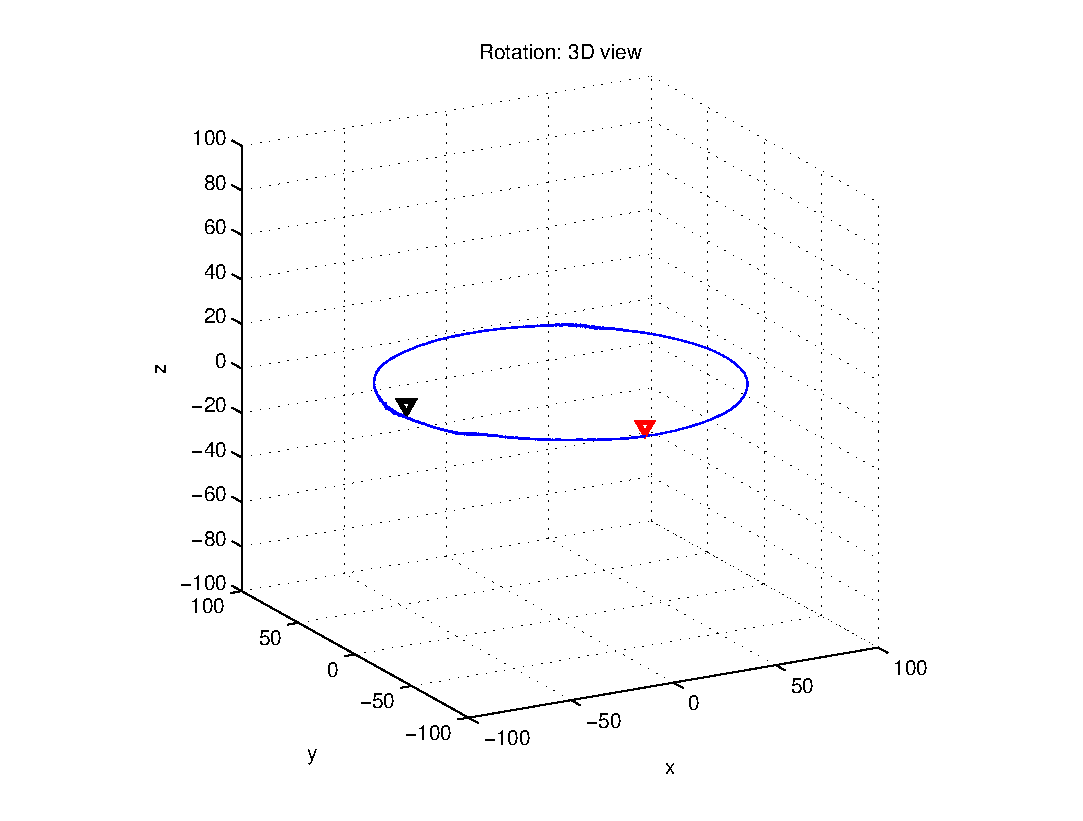
\includegraphics[width=0.45\textwidth]{include/linguometer/images/int_ex_1.eps}}
	\hspace{0.05\textwidth}
	\subfigure[\label{fig:linguometer:technical:interference:ex:2}]
	{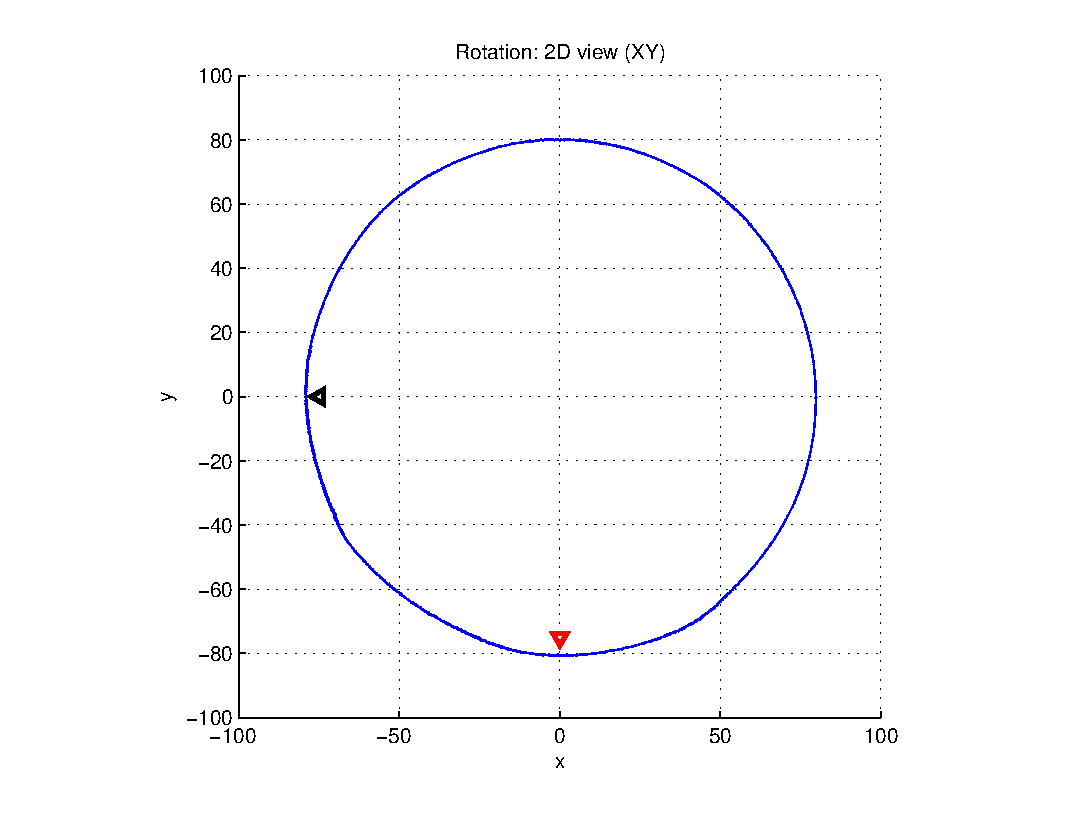
\includegraphics[width=0.45\textwidth]{include/linguometer/images/int_ex_2.eps}}
	
	\subfigure[\label{fig:linguometer:technical:interference:ex:3}]
	{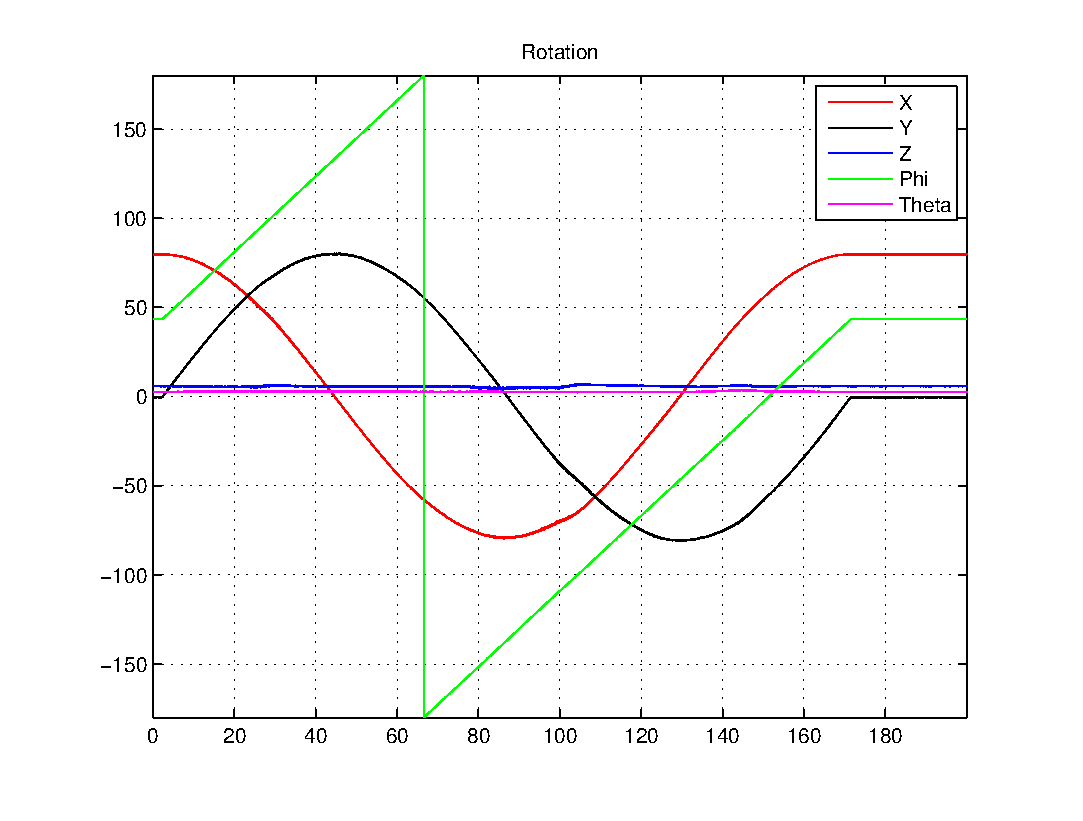
\includegraphics[width=0.45\textwidth]{include/linguometer/images/int_ex_3.eps}}
	\hspace{0.50\textwidth}
	
	\caption[Articulograph sensor rotation]{\textbf{Articulograph sensor
	rotation}: (a) tridimensional view of the rotation of a single sensor
	attached to the AG500 magazines used for calibration. 
	(b) Bidimensional projection (top view) of the previous plot.
	(c) This plot shows the 5DOF acquired by the means of electromagnetic 
	articulography. Three cartesian coordinates (X, Y and Z) and two spherical
	coordinates (Azimuth Tetha and elevation Phi).
	Notes: the red triangle indicates the sensor starting point with respect
	to the XY plane (0 seconds). 
	The black triangle indicates the position of the ultrasonograpic 
	transducer (XY plane).
	The radius of the rotation measures 80 mm while the height at which 
	the rotation takes place measures 6.5 mm. The Theta angle measures circa
	5 $^{\circ}$ and the Phi angle varies during the rotation.
	}
	\label{fig:linguometer:technical:interference:ex}
\end{figure}
% ---------------------------------------------------------------------------- %

In this section, two different tests are presented. The first one is a
bidimensional test the author executed to verify the possibility of
recording  simultaneously with the articulograph and the ultrasound system.
The second test provides an example of how the articulograph kinesthetic data is
validated during the investigations.

% ---------------------------------------------------------------------------- %
\subsubsection{Ad-hoc bidimensional test}
% ---------------------------------------------------------------------------- %
Regarding the first test, three different cases are discussed.
In the first case, four articulograph sensors are calibrated without the 
ultrasonograpic transducer inside the frame of reference, thus
providing a reference condition being the articulograph used in the best
possible context (e.g.: the electromagnetic interference caused by the
ultrasonograpic transducer is absent).
The four sensors used for the investigation are left on the magazine used during
the calibration process, and the AG500 Circal is rotated by 360$^{\circ}$.
The amplitudes are acquired and the positions are computed as described in
Section~\ref{sec:linguometer:instrumentation:ag}.
Figure~\ref{fig:linguometer:technical:interference:ex} provides an example
of the rotation of a sensor.
Although this description is not strictly necessary, it turns useful to 
discuss a problem that affects the 
calculation of the positions starting from the amplitudes recorded with the
articulograph AG500.

% ---------------------------------------------------------------------------- %
\begin{figure}
	\centering
	\subfigure[\label{fig:linguometer:technical:interference:isd:1}]
	{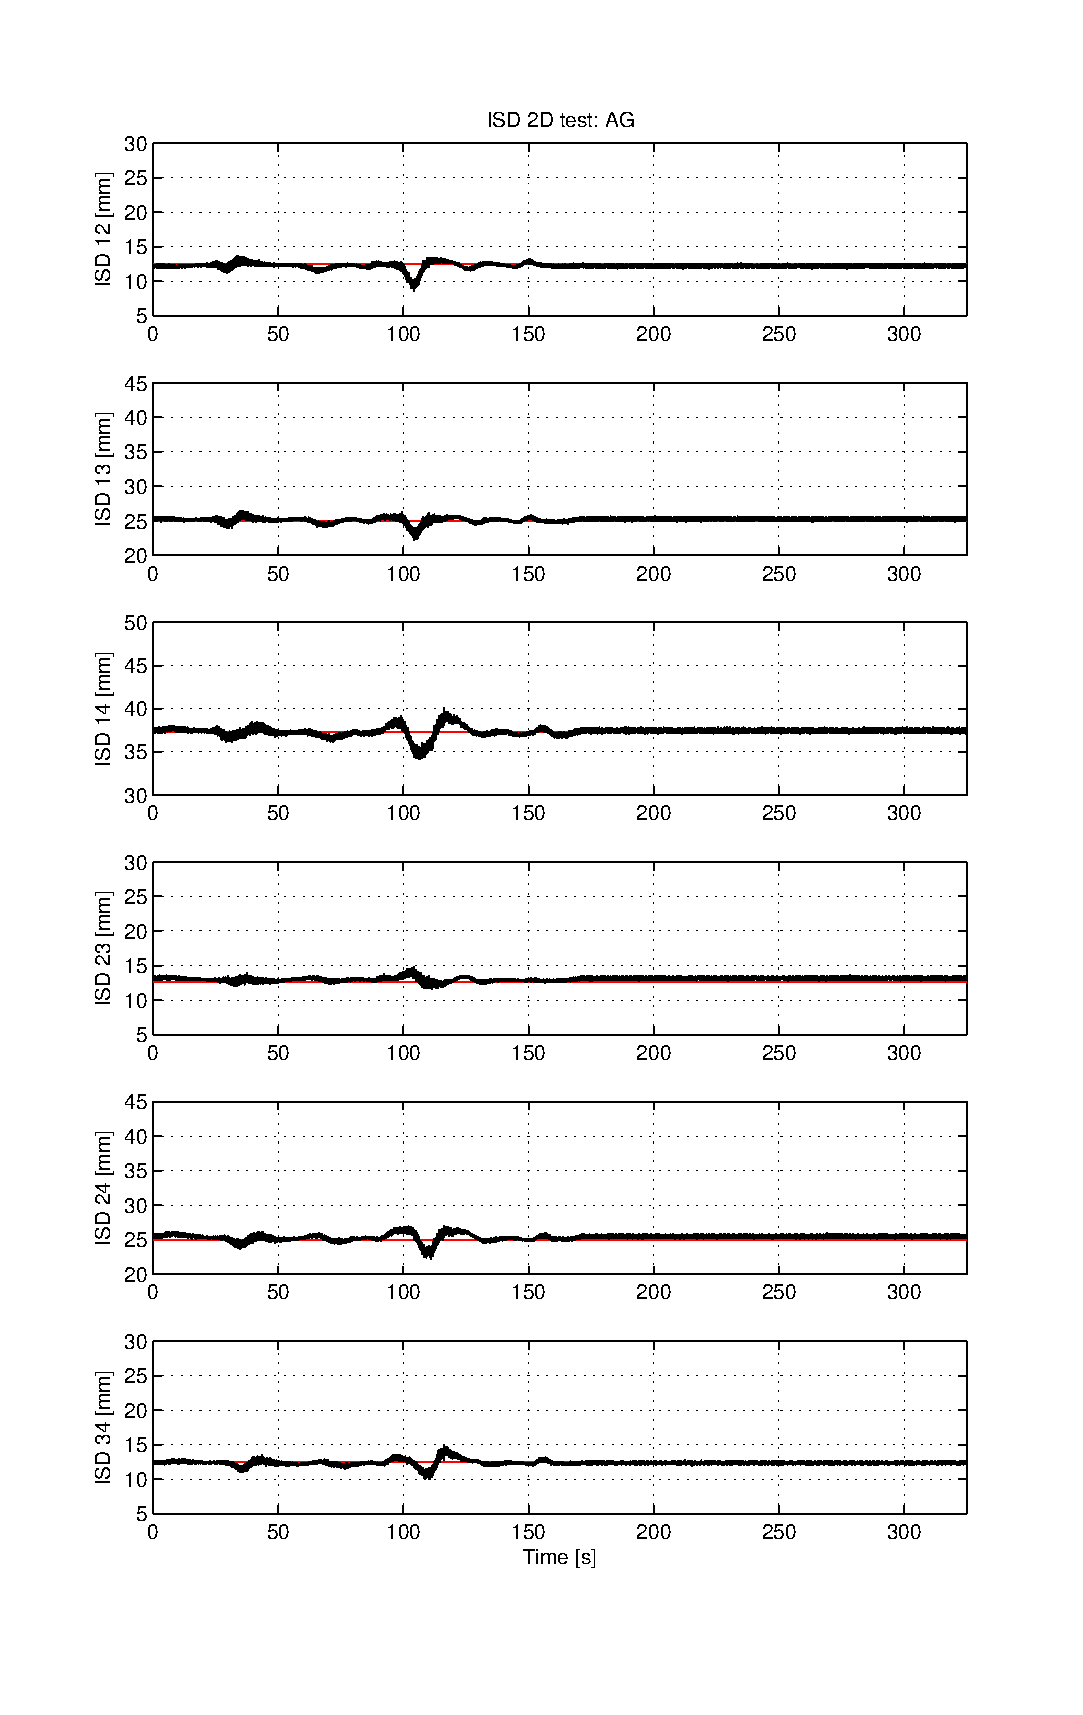
\includegraphics[width=0.35\textwidth]{include/linguometer/images/int_isd3d_1.eps}}
	\subfigure[\label{fig:linguometer:technical:interference:isd:2}]
	{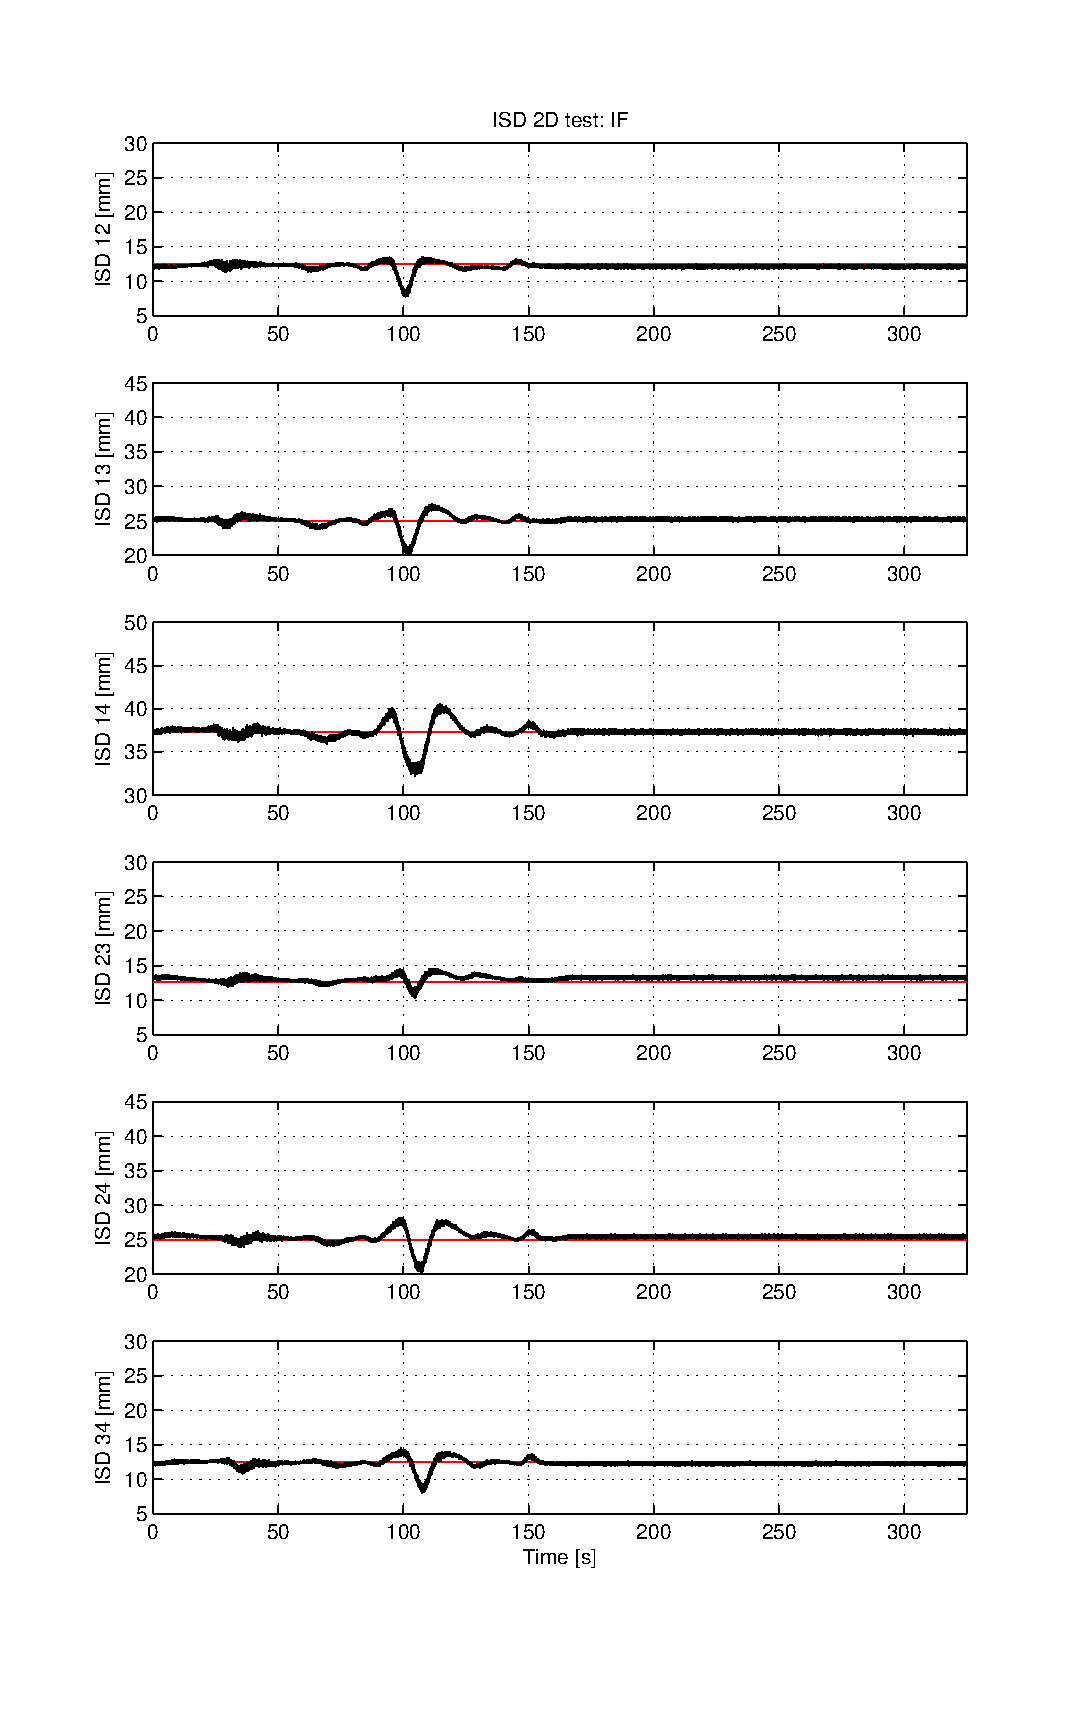
\includegraphics[width=0.35\textwidth]{include/linguometer/images/int_isd3d_2.eps}}

	\subfigure[\label{fig:linguometer:technical:interference:isd:3}]
	{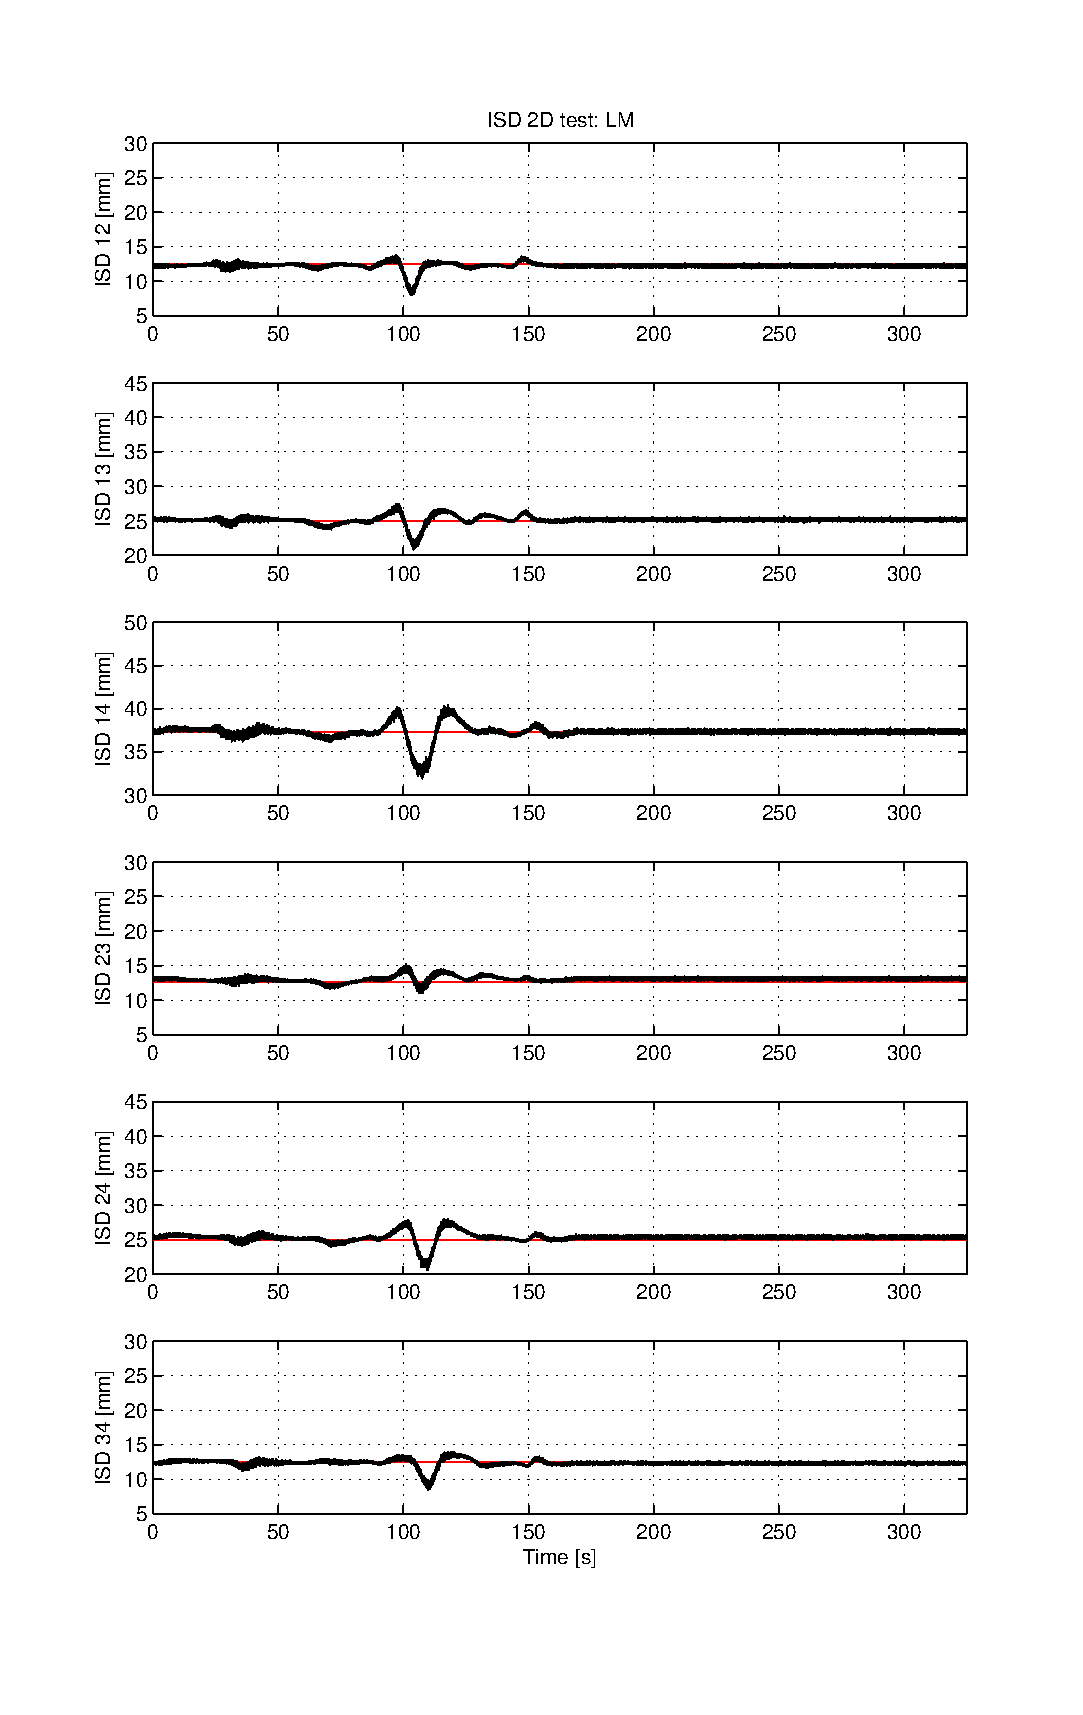
\includegraphics[width=0.35\textwidth]{include/linguometer/images/int_isd3d_3.eps}}
	\hspace{0.35\textwidth}

	\caption[ISD results (ad-hoc test, XYZ)]{\textbf{ISD results (ad-hoc test, XYZ)}:
	ISDs calculated considering the three Cartesian coordinates of each 
	acquired sample (X, Y and Z).
	(a) AG test, (b) IF test and (c) LM test.
	Red plots: ISD between sensors 1 and 2. Black plots: ISD between sensors 2
	and 3. Blue plots: ISD between sensors 3 and 4. 
	Notes: ISD scale in millimiters, time scale in seconds. The revolution of
	the circal starts between 0 and 1.5 seconds and ends approximately at 170
	seconds. From 170 seconds to the end of the acquisition, the sensors remain
	still in the initial position.
	}
	\label{fig:linguometer:technical:interference:isd}
\end{figure}
% ---------------------------------------------------------------------------- %

In the second case, the ultrasonograpic transducer is placed inside the
EMA-Cube, and the sensors are rotated again, as explained for the first case.
Finally, in the third case the articulograph is calibrated in the ``Linguometer
configuration'', that is, with the ultrasonograpic transducer inside the
Ema-Cube.
As in the two preceding cases, a revolution of the AG500 Circal is executed.

To sum up, three different cases are here presented. 
The first one deals with the articulograph in the best possible recording
conditions, that is without any interfering object inside the frame of 
reference (\emph{AG test}).
In the second case, the worst possible condition is created. In fact, the
ultrasonograpic probe is placed inside the frame of reference without an
appropriate calibration of the articulograph (\emph{IF test}).
If the ultrasonograpic transducer generates a perturbation of the
electromagnetic field, this particular configuration should lead to 
trajectories that diverge from the reference one.
If the interference can be compensated by the means of calibration, then the
third case (\emph{LM test}) should prove this hypothesis.
All the tests rely on the idea that, being the sensors fixed to the magazines,
the euclidean distance between any pair of those should remain constant during
the revolution of the Circal.

Figure~\ref{fig:linguometer:technical:interference:isd} shows the computed
ISDs for the three cases respectively.
At least for the first case (\emph{AG test}), the ISD values should remain
constant along the whole rotation, but unfortunately this is not true.
In fact, the ISD values remain constant only at the end of the rotation, when
the sensors are kept in a fixed position nearby the starting point
(e.g.: the red triangle in 
Figure~\ref{fig:linguometer:technical:interference:ex}).
The author, worried about the unexpected results, questioned Carstens
Medizinelektronik GmbH. Apparently, the problem is well known and Carstens
Medizinelektronik GmbH is working on a solution. Furthermore, no literature or
official documentation has been released about the odd behavior.\\
As a consequence, the author decided to quote the answer provided by Carstens
Medizinelektronik GmbH:
\begin{quote}
Please have a look to the circal run and switch on only the "Z" coordinate.
Here you can see that the value for Z has a stronger deviation in 2 points.
Without any error, the Z should appear as a line because the value of Z does 
not change during a revolution of the circal.
We suspect that there are points in the 5 dimensional space where a change in x,
y, z, phi and theta will result in a amplitude change that is lower than the 
error tolerance.
We call this "weak points" because at this position and orientation there is no 
strong relationship between measured amplitudes and calculated position and 
orientation.
In other words: a large change in the position and orientation will cause a 
small change in the measured amplitudes.
So we can not guarantee to calculate a correct position and orientation at all 
possible 5 dimensional locations.
During speech movement it seems that the sensor fortunately runs very quick 
through weak points, so that the program does not get lost.
At this point we do not have all complete answers to this problem. 
We have some observations and will continue to investigate this circumstances.
At the moment we have the strategy to reduce the measurement error as far as 
possible.
\begin{flushright}
{\small Bahne Carstens\footnote{Bahne Cartsten, Cartsens Medizinelektronik GmbH,
April 12, 2007.}}
\end{flushright}
\end{quote}
Figure~\ref{fig:linguometer:technical:interference:ex:3} shows the trajectories 
of the five coordinates characteristic to the AG500 Circal revolution while
Figure~\ref{fig:linguometer:technical:interference:exz} shows a zoomed version
of the previous plot. 
The two regions of increased variance pointed out by Cartsens Medizinelektronik
GmbH are clearly visible in the 20-40 seconds and in the 80-100 seconds
intervals respectively.
% ---------------------------------------------------------------------------- %
\begin{figure}[!ht]
\centering

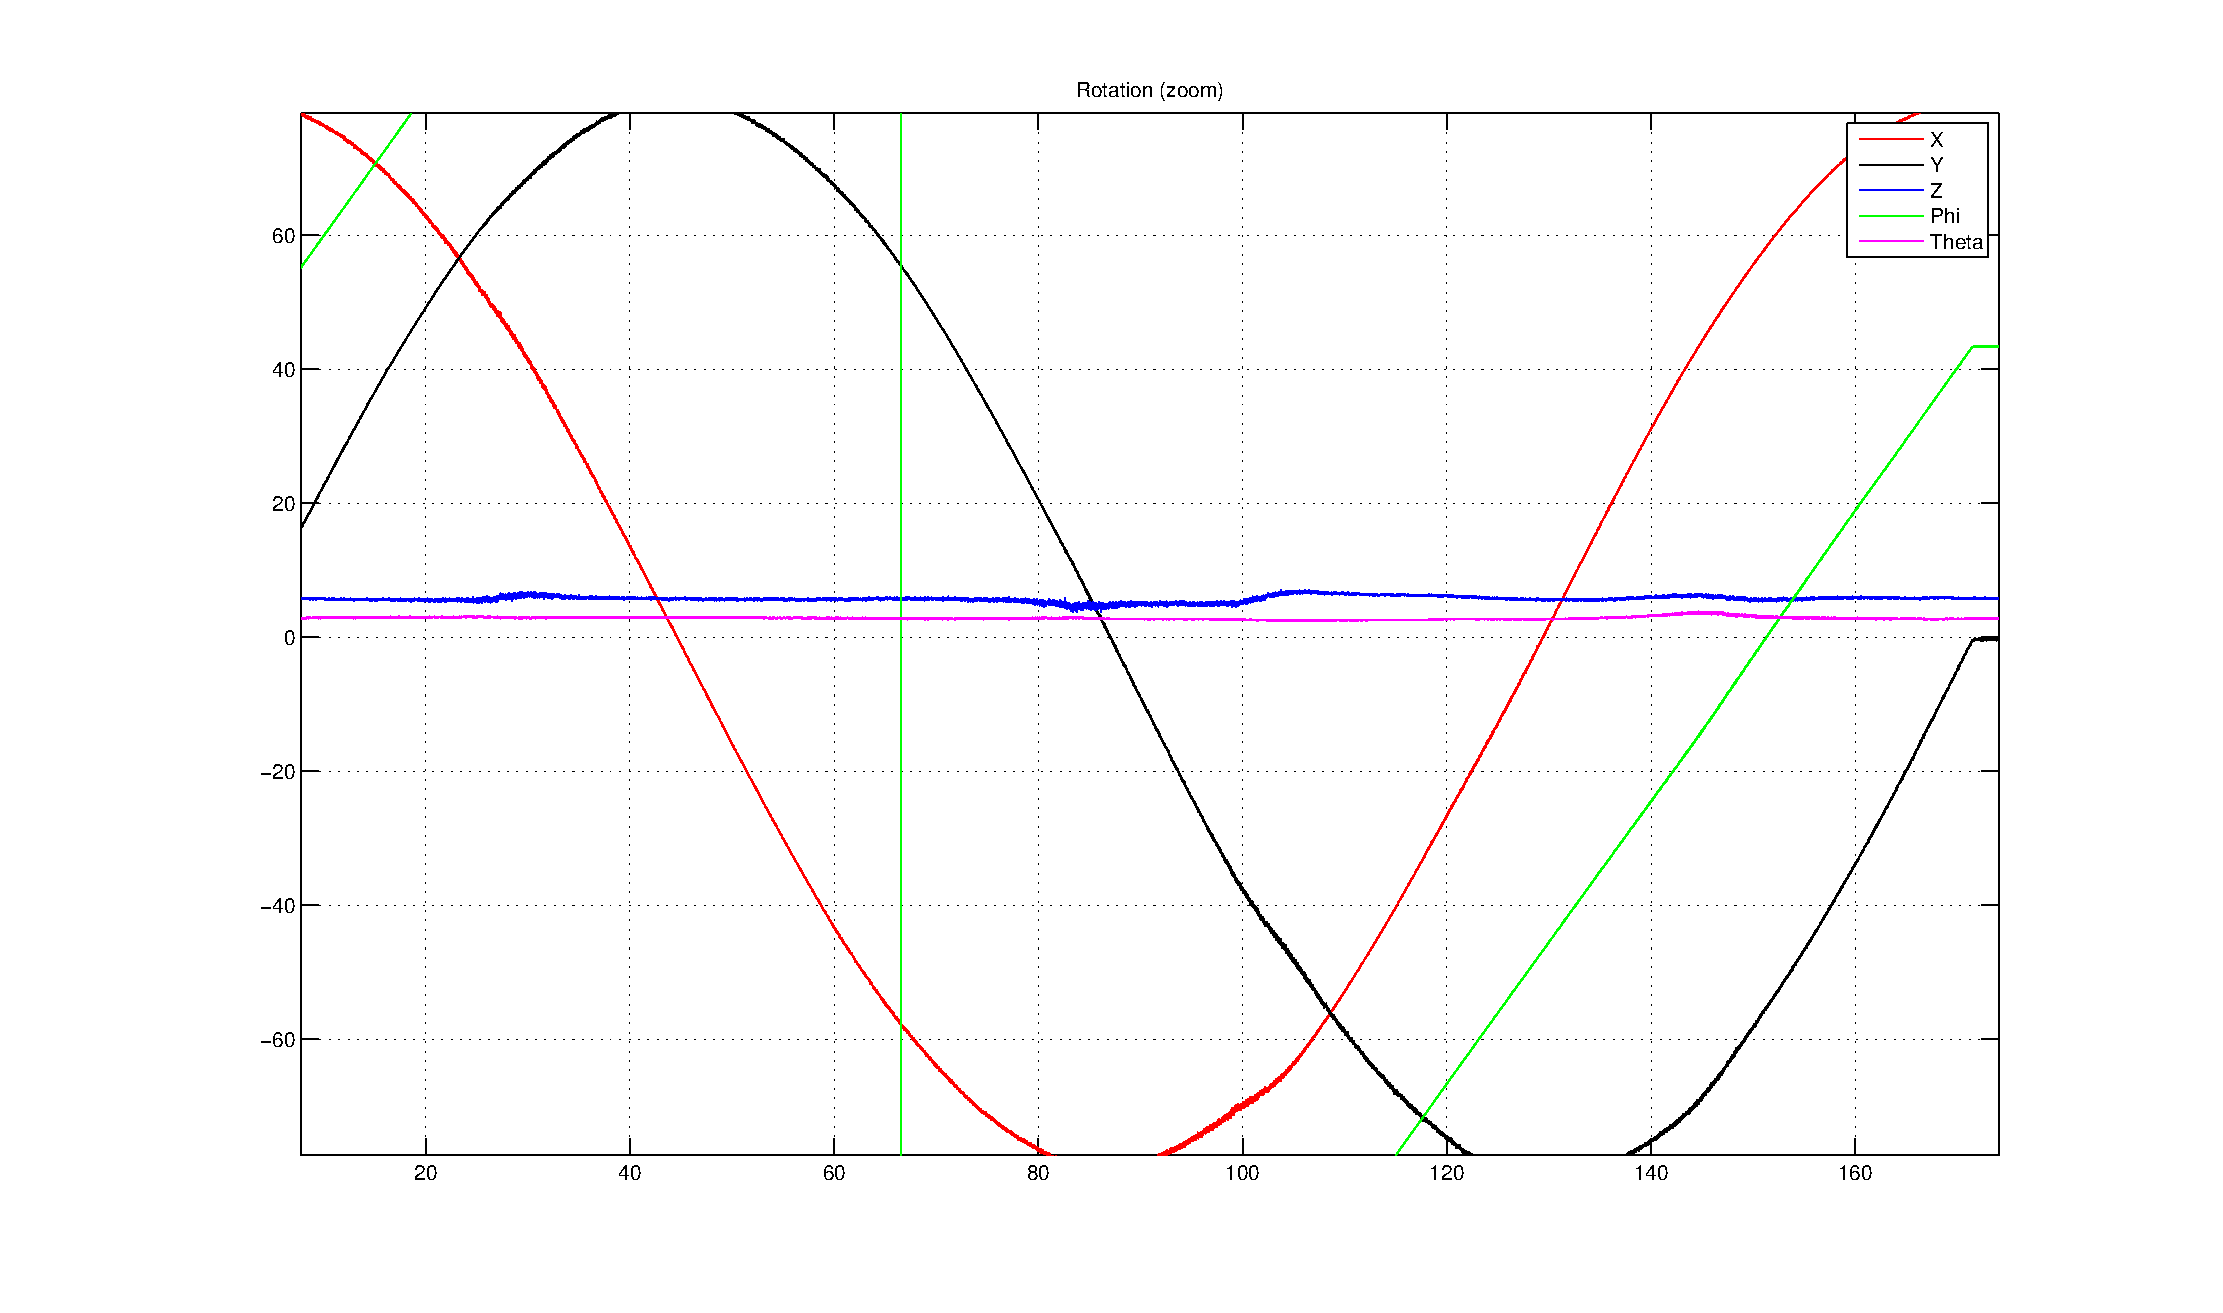
\epsfig{file=include/linguometer/images/int_ex_4.eps,width=1.00\textwidth}
	\caption[Articulograph sensor trajectory error]{\textbf{Articulograph
	sensor trajectory error}: 
	The two regions where the Z coordinate variance increases 
	are clearly visible in the 20-40 seconds and in the 80-100 seconds 
	intervals respectively.}
	\label{fig:linguometer:technical:interference:exz}
\end{figure}
% ---------------------------------------------------------------------------- %

% ---------------------------------------------------------------------------- %
\begin{figure}
	\centering
	\subfigure[\label{fig:linguometer:technical:interference:isd2:1}]
	{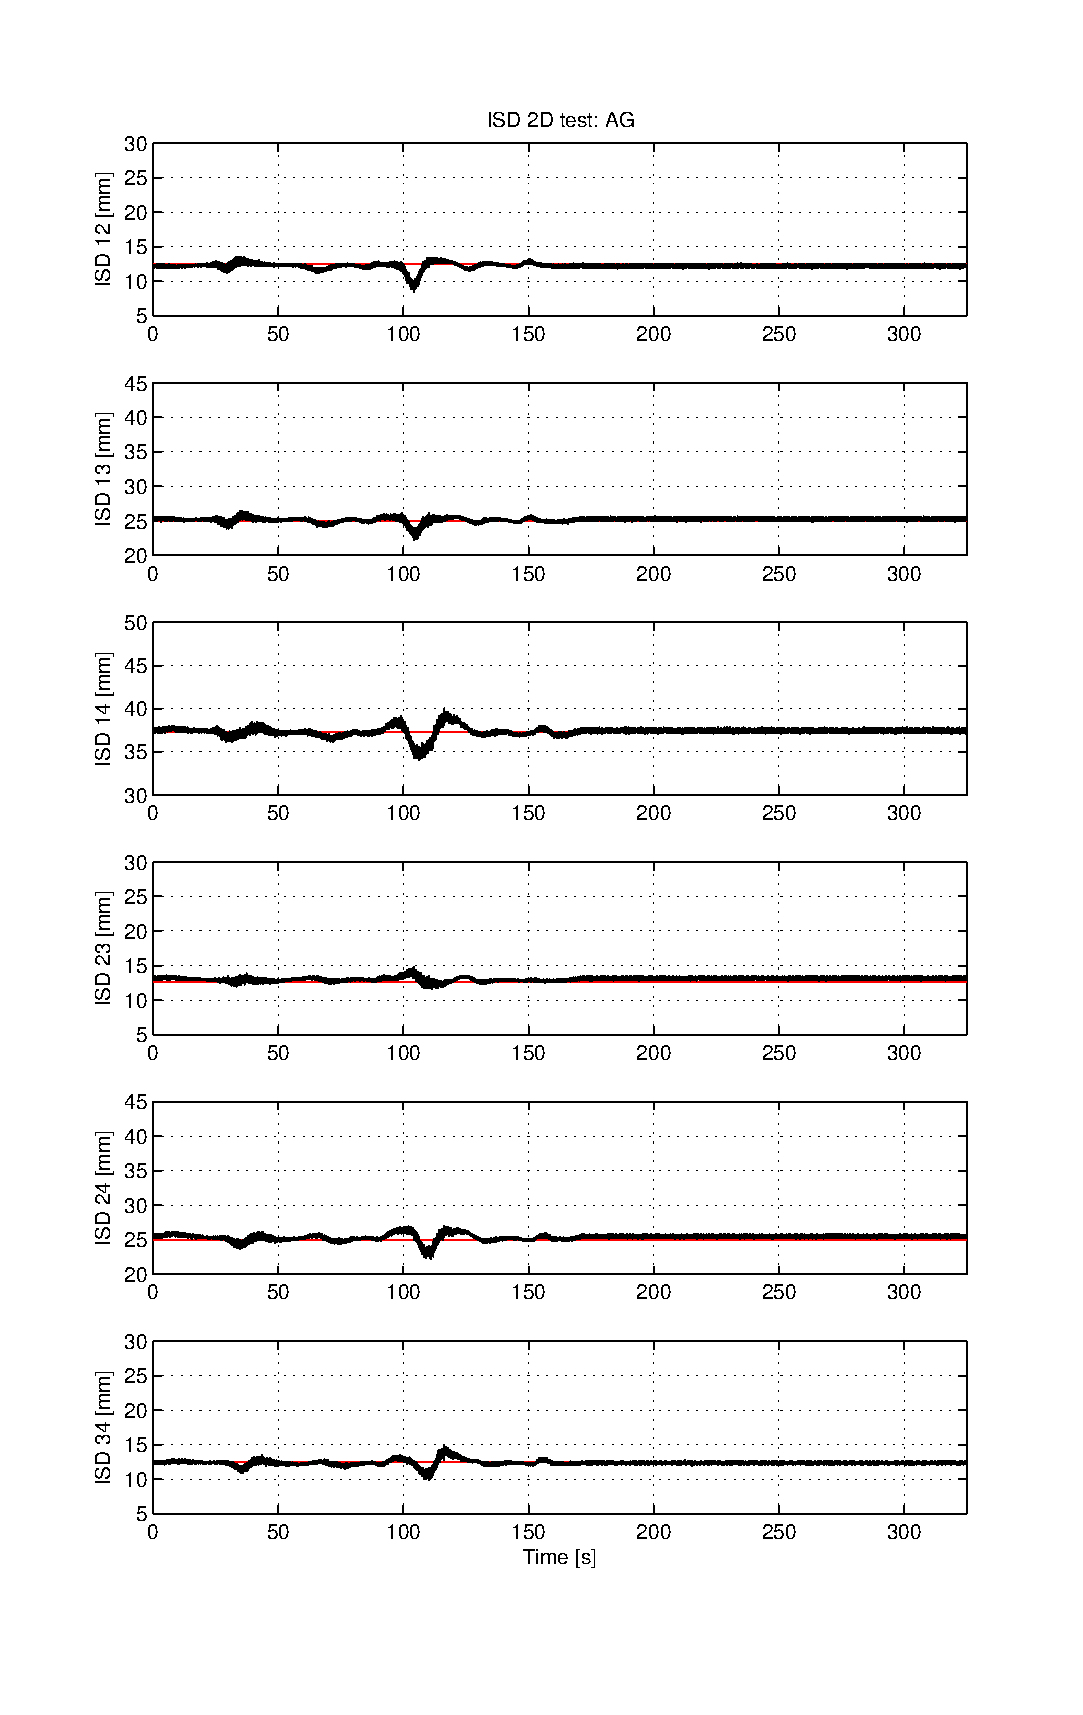
\includegraphics[width=0.35\textwidth]{include/linguometer/images/int_isd2d_1.eps}}
	\subfigure[\label{fig:linguometer:technical:interference:isd2:2}]
	{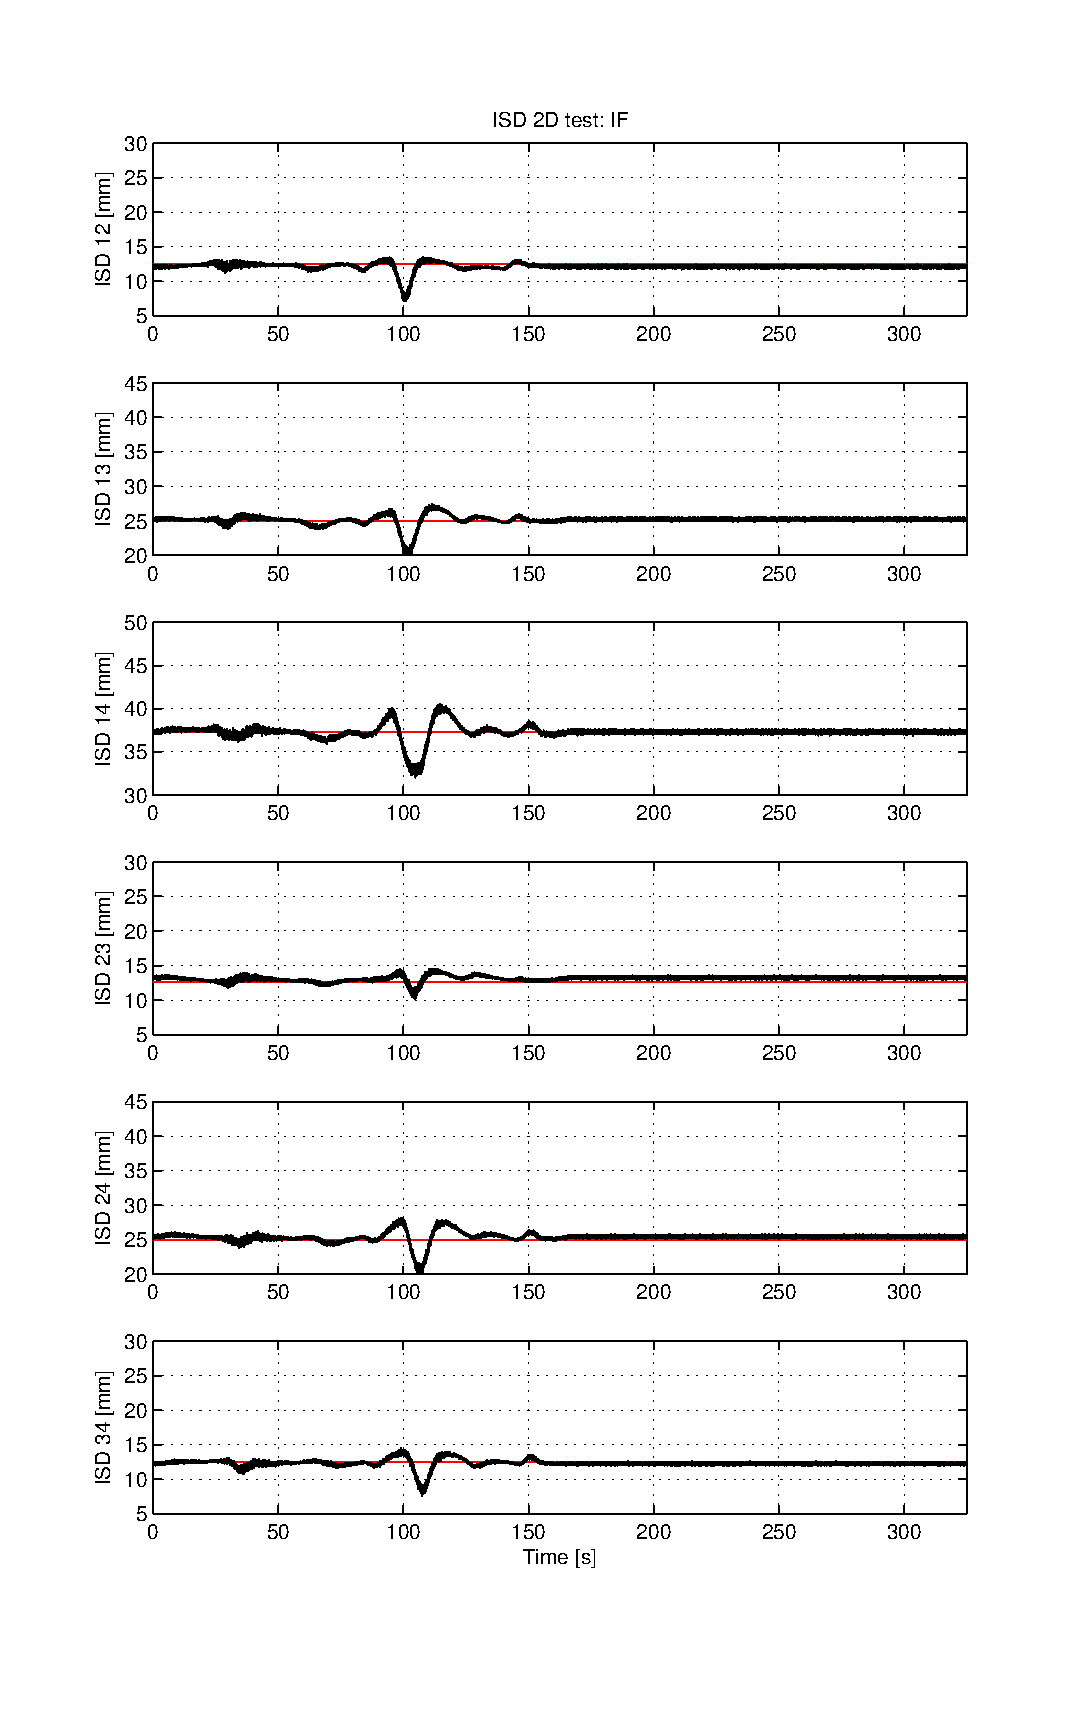
\includegraphics[width=0.35\textwidth]{include/linguometer/images/int_isd2d_2.eps}}

	\subfigure[\label{fig:linguometer:technical:interference:isd2:3}]
	{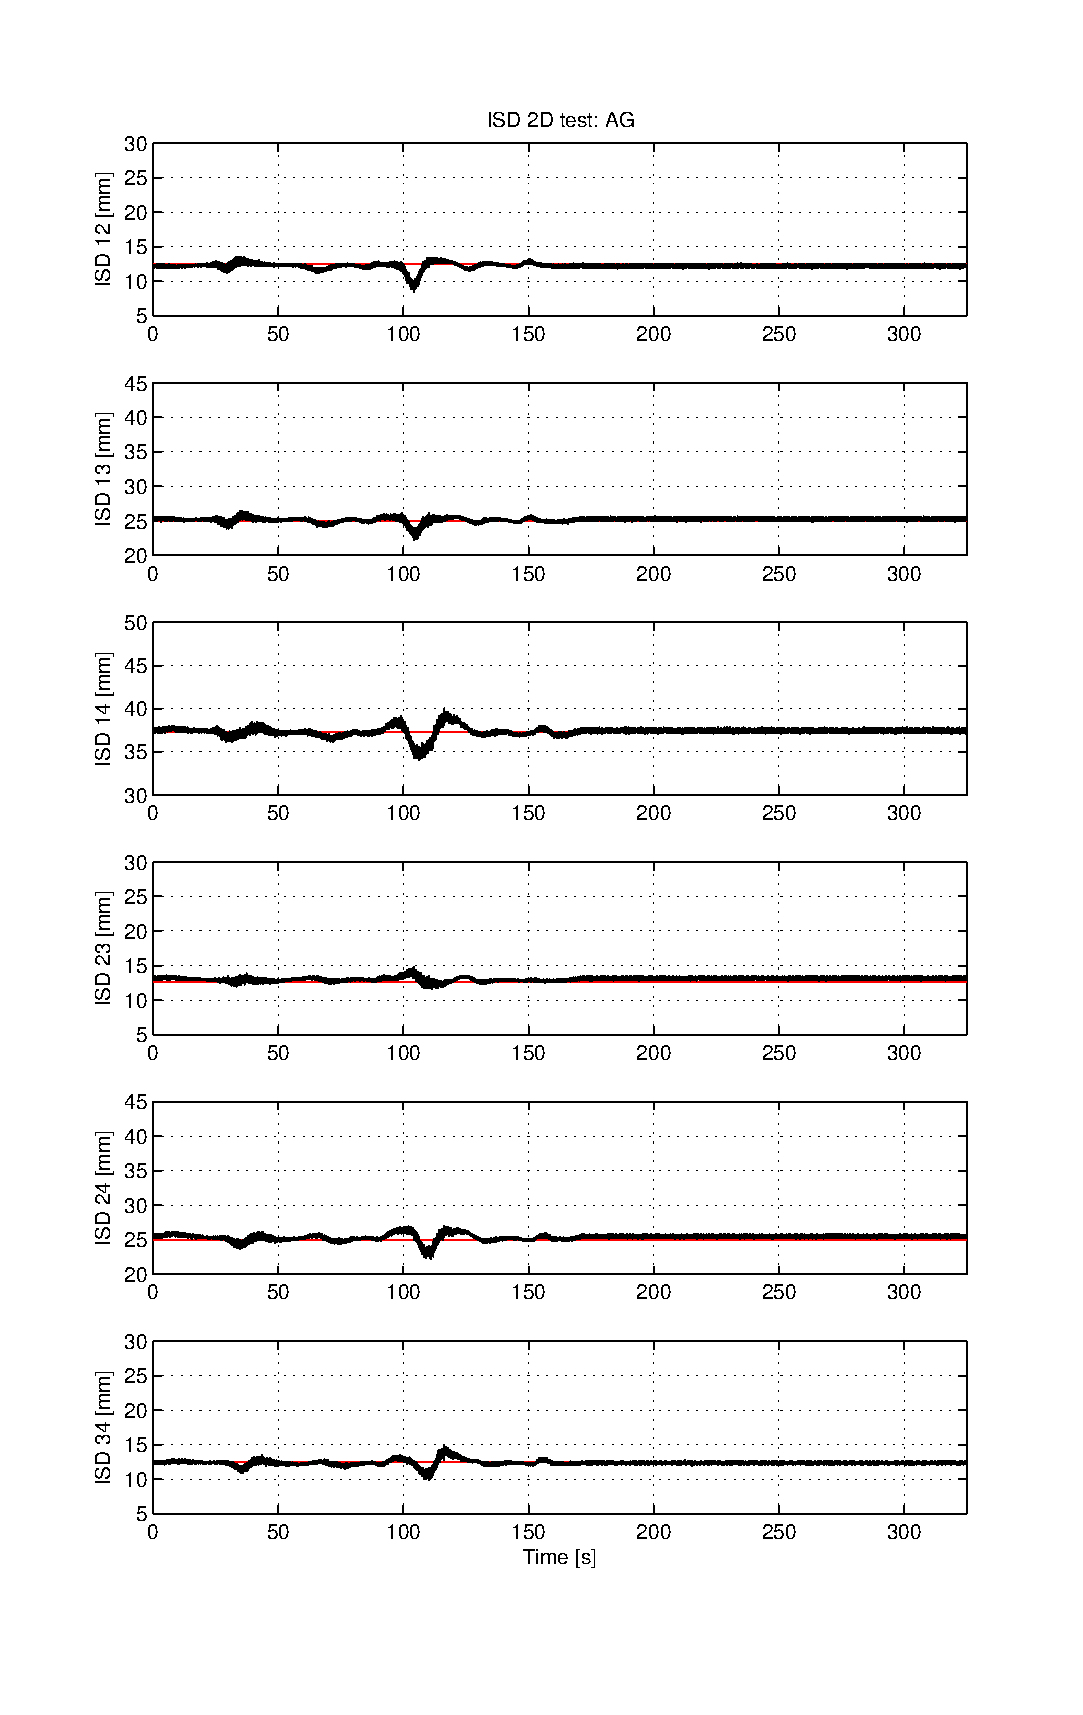
\includegraphics[width=0.35\textwidth]{include/linguometer/images/int_isd2d_3.eps}}
	\hspace{0.35\textwidth}
	
	\caption[ISD results (ad-hoc test, XY)]{\textbf{ISD results (ad-hoc test, XY)}:
	ISDs calculated considering the first two Cartesian coordinates of each 
	acquired sample (X and Y).
	(a) AG test, (b) IF test and (c) LM test.}
	\label{fig:linguometer:technical:interference:isd2}
\end{figure}
% ---------------------------------------------------------------------------- %

According to Carstens Medizinelektronik GmbH, the problem affects only the Z
coordinate. If this is the case, then the ISDs calculated by the means of
euclidean distance using just the X and Y coordinates should prove to be
constant.
Again, this is not the case, as shown in 
Figure~\ref{fig:linguometer:technical:interference:isd2}.
Looking closer at Figure~\ref{fig:linguometer:technical:interference:exz}, the
reader can easily notice that, inside the problematic intervals, the variance 
increases also for the X and Y coordintates. Furthermore the X and Y curves are
distorted nearby the regions where the Z variance increases.
Table~\ref{tab:linguometer:technical:isd:test} reports the statistical results
of the ISD measures in both the tridimensional (X, Y and Z) and bidimensional
(X and Y) cases.
%maybe talk about the discontinuity problem

The problems introduced in the preceding paragraphs does not allow the author to
draw any provable conclusion about the topic of interference compensation.
In fact, the the algorithm developed by Carstens Medizinelektronik GmbH 
does not compute correcly the trajectory of the sensors in the simplest case 
(\emph{AG test}), where a simple rotation of the Circal is executed. 
Furthermore, the rotation of the Circal itself is fundamental for the
calibration of the AG500 articulograph. Those two issues are not negligible and
surely made the whole interference compensation procedure more complicated than
expected.
The fact that the ISDs measured in the bidimensional case (X and Y) are not
constant reveal that probably the algorithm fails calculating all the three
Cartesian coordinates and not just Z, as suggested by Carstens
Medizinelektronik GmbH.

\begin{table}[htbp]
  \begin{center}
  \begin{scriptsize}
	\begin{tabular}{|c|c|cc|cc|cc|}
	  \hline
	   & \textbf{Exp.} & \misds{2D} & \sisds{2D} & \misds{3D} & \sisds{3D}\\
	  \hline
	  AG-12 & 12.53 & 12.21 & 0.38 & 12.20 & 0.39\\
	  AG-13 & 25.00 & 25.17 & 0.31 & 25.17 & 0.31\\
	  AG-14 & 37.30 & 37.37 & 0.50 & 37.36 & 0.50\\
	  AG-23 & 12.55 & 13.05 & 0.25 & 13.04 & 0.25\\
	  AG-24 & 25.00 & 25.36 & 0.43 & 25.36 & 0.43\\
	  AG-34 & 12.53 & 12.38 & 0.35 & 12.37 & 0.35\\
	  \hline
	  IF-12 & 12.53 & 12.01 & 0.56 & 12.02 & 0.61\\
	  IF-13 & 25.00 & 25.54 & 0.68 & 25.78 & 0.69\\
	  IF-14 & 37.30 & 37.08 & 0.84 & 37.01 & 0.87\\
	  IF-23 & 12.55 & 13.66 & 0.39 & 13.34 & 0.41\\
	  IF-24 & 25.00 & 25.78 & 0.75 & 25.23 & 0.77\\
	  IF-34 & 12.53 & 12.67 & 0.60 & 12.53 & 0.62\\
	  \hline
	  LM-12 & 12.53 & 12.21 & 0.47 & 12.20 & 0.49\\
	  LM-13 & 25.00 & 25.13 & 0.56 & 25.13 & 0.56\\
	  LM-14 & 37.30 & 37.30 & 0.80 & 37.30 & 0.81\\
	  LM-23 & 12.55 & 13.03 & 0.35 & 13.02 & 0.35\\
	  LM-24 & 25.00 & 25.32 & 0.65 & 25.31 & 0.67\\
	  LM-34 & 12.53 & 12.36 & 0.46 & 12.35 & 0.49\\
	  \hline
  \end{tabular}
  \end{scriptsize}
  \end{center}
	\caption[ISD results (ad-hoc test)]{\textbf{ISD results (ad-hoc test)}:
	the last two rows values are in milliseconds. Where not
	specified, values are in samples.
	Note: \misds{2D} and \sisds{2D}: average and standard deviation values for 
	the bidimensional case;
	\misds{3D} and \sisds{3D}: average and standard deviation values for 
	the tridimensional case. 
	}
 \label {tab:linguometer:technical:isd:test}
\end{table}

An additional issue does need to be discussed in this context. 
The spatial arrangement of the reference coils forced the author to use the
articulograph back-to-front.
In fact, the subjects stare toward the negative X
axis (Figure~\ref{fig:linguometer:technical:interference:ex:2} and
Figure~\ref{fig:experiments:exp}).
On the contrary, the articulograph was designed so that the subjects look
toward the positive X direction during the investigations.
As a consequence of the back-to-front usage of the articulograph,
the subject's articulators were positioned really close to the zone
characterized by the error previously described.
The question that arises from the presented discussion addreessee the possibily
that inside the frame of reference of the articulograph exists a volume where
the positions of the sensors can not be properly calculated.
Furthermore, the articulograph AG500 does not provide by itself consistent
results. In this context, the author believes that a solution to the
interference compensation problem could be only provided by running tests using
an optical tracker or similarly reliable device.

Before introducing the validation procedure used during the experiments, few
conclusion should be drawn starting from the results condensed in 
Table~\ref{tab:linguometer:architecture:sig:delay}.
The table shows the ISD average and standard deviation values for each couple
of sensors, for the three test cases presented earlier in this Section 
(e.g: \emph{AG}, \emph{IF} and \emph{LM test}).
Furthermore, the values are shown both for the bidimensional
computation of the ISD values (2D: X and Y) and for the tridimensional one (3D:
X, Y and Z).\\
In the case of \emph{AG} and \emph{LM test}, the average and the standard
deviation values appear to be quite similar, albeit the variance is generally
higher in the \emph{LM} case.
Regarding the \emph{IF} case, the variance is higher than in the remaining two
cases and the mean ISD values do not resemble what shown for the \emph{AG} case.
Apparently the procedure used to compensate the interference works.
As a matter of fact, the average and the standard deviation values in the
\emph{LM} case resemble what shown for the \emph{AG} case.
On the other hand, the values shown for the \emph{IF} case are quite 
dissimilar to the \emph{AG} reference ones.
Interestingly, the \emph{LM} case shows an higher variance, probably because
the \emph{LM} problem is harder to solve than the AG one due the presence of
the interfering object.
% ---------------------------------------------------------------------------- %
\subsubsection{Validation of the recorded data}
% ---------------------------------------------------------------------------- %
The aim of the previous Section was to introduce the reader to the simple
procedure adopted for compensating the effect of placing the ultrasonograpic
transducer directly inside the AG500 frame of reference.
In this section the procedure used to validate the 
kinesthetic data recorded during the investigations is discussed.
Figure~\ref{fig:linguometer:technical:glasses:0} shows  the positions of the
reference sensors used for head movement compensation (sensor 10, 11 and 12).
Furthermore, sensor 6 is glued on the upper teeth, thus it is occluded by the 
\emph{labia majora}~(Figure~\ref{fig:experiments:map}).

% ---------------------------------------------------------------------------- %
\begin{figure}
	\centering
	  \subfigure[\label{fig:linguometer:technical:glasses:0}]
		{\includegraphics[width=0.25\textwidth]{include/linguometer/images/glasses_0.tps}}
		\hspace{0.05\textwidth}
	  \subfigure[\label{fig:linguometer:technical:glasses:1}]
		{\includegraphics[width=0.25\textwidth]{include/linguometer/images/glasses_1.tps}}
		\hspace{0.05\textwidth}
	  \subfigure[\label{fig:linguometer:technical:glasses:2}]
		{\includegraphics[width=0.25\textwidth]{include/linguometer/images/glasses_2.tps}}
	\caption[Head movement compensation glasses]{\textbf{Head movement
	compensation glasses}: (a) position of the reference sensors (10, 11 and 12)
	and of the upper teeth sensor. Being the teeth constraint to the head,
	measuring the ISD values between sensor 6 and the sensors on the glasses
	turns out to be useful for detecting the motion of the latter. It may happen
	that the glasses wear by the subject slide towards the tip of the nose (b
	and c). Refer to Figure~\ref{fig:experiments:map} for a complete sensor
	map.}
	\label{fig:linguometer:technical:glasses}
\end{figure}
% ---------------------------------------------------------------------------- %

Being the glasses a rigid body, the ISDs between the reference
sensors should remain constant during the whole duration of an experiment.
As already said, each experiment is made up by nine different sequences. 
Figure~\ref{fig:linguometer:technical:isd:example} shows three cases used as
example to describe how the kinesthetic data is validated.

\begin{table}[htbp]
  \begin{center}
  \begin{scriptsize}
	\begin{tabular}{|c|c|cc|cc|cc|}
	  \hline
	  \textbf{Exp}. & \textbf{Seq.} & \misd{6}{10} & \sisd{6}{10} & \misd{6}{11} & \sisd{6}{11} & \misd{6}{12} & \sisd{6}{12}\\
	  \hline
	  0 & 1 & 84.08 & 1.16 & 84.59 & 0.25 & 48.82 & 0.32\\
		& 2 & 85.41 & 0.91 & 84.64 & 0.27 & 49.01 & 0.32\\
		& 3 & 84.91 & 0.97 & 84.25 & 0.26 & 48.90 & 0.31\\
		& 4 & 85.28 & 0.70 & 84.17 & 0.29 & 48.84 & 0.45\\
		& 5 & 85.04 & 1.27 & 84.02 & 0.32 & 48.86 & 0.36\\
		& 6 & 85.60 & 1.63 & 83.59 & 0.32 & 48.48 & 0.34\\
		& 7 & 86.02 & 1.25 & 83.43 & 0.34 & 48.42 & 0.32\\
		& 8 & 86.32 & 0.74 & 83.20 & 0.34 & 48.43 & 0.34\\
		& 9 & 86.19 & 1.36 & 83.94 & 0.48 & 48.93 & 0.42\\
	  \hline
	  1 & 1 & 90.07 & 0.25 & 88.47 & 0.47 & 48.63 & 0.53\\
		& 2 & 90.05 & 0.21 & 88.41 & 0.48 & 48.63 & 0.56\\
		& 3 & 90.09 & 0.25 & 88.27 & 0.49 & 48.58 & 0.55\\
		& 4 & 90.27 & 0.26 & 88.55 & 0.54 & 48.93 & 0.63\\
		& 5 & 89.92 & 0.17 & 88.06 & 0.42 & 48.57 & 0.51\\
		& 6 & 89.80 & 0.16 & 88.11 & 0.39 & 48.70 & 0.47\\
		& 7 & 89.92 & 0.15 & 88.18 & 0.33 & 48.75 & 0.42\\
		& 8 & 89.88 & 0.14 & 88.06 & 0.34 & 48.66 & 0.42\\
		& 9 & 89.86 & 0.18 & 88.14 & 0.38 & 48.80 & 0.45\\
	  \hline: 
	  4 & 1 & 87.65 & 0.47 & 88.13 & 0.58 & 50.18 & 0.58\\ 
		& 2 & 85.81 & 0.42 & 86.10 & 0.47 & 48.76 & 0.48\\ 
		& 3 & 84.26 & 0.38 & 84.63 & 0.36 & 47.78 & 0.35\\ 
		& 4 & 80.02 & 0.40 & 80.45 & 0.41 & 45.36 & 0.36\\ 
		& 5 & 79.02 & 0.39 & 79.52 & 0.32 & 44.87 & 0.27\\ 
		& 6 & 87.69 & 0.25 & 87.78 & 0.28 & 50.17 & 0.28\\
		& 7 & 87.11 & 0.23 & 87.46 & 0.22 & 49.80 & 0.29\\
		& 8 & 86.62 & 0.21 & 87.20 & 0.25 & 49.62 & 0.24\\
		& 9 & 84.62 & 0.59 & 85.02 & 0.47 & 48.09 & 0.32\\
	  \hline
	  \textbf{Exp}. & \textbf{Seq.} & \misd{11}{12} & \sisd{11}{12} & \misd{10}{11} & \sisd{10}{11} & \misd{10}{12} & \sisd{10}{12}\\
	  \hline
	  0  & 1 & 48.08 & 0.20 & 43.58 & 3.84 & 72.04 & 3.18\\
		 & 2 & 48.10 & 0.22 & 48.54 & 4.90 & 76.02 & 3.40\\
		 & 3 & 47.93 & 0.21 & 44.68 & 4.18 & 73.54 & 3.19\\
		 & 4 & 47.86 & 0.19 & 47.92 & 3.85 & 75.74 & 2.77\\
		 & 5 & 47.83 & 0.22 & 47.83 & 4.87 & 75.64 & 3.65\\
		 & 6 & 47.72 & 0.28 & 51.98 & 6.24 & 78.38 & 4.68\\
		 & 7 & 47.66 & 0.30 & 54.52 & 5.82 & 80.16 & 4.10\\
		 & 8 & 47.75 & 0.54 & 56.82 & 3.30 & 82.00 & 2.33\\
		 & 9 & 47.74 & 0.31 & 55.18 & 5.71 & 80.58 & 4.00\\
	  \hline
	  1 & 1 & 48.21 & 0.15 & 57.89 & 0.15 & 79.41 & 0.22\\
		& 2 & 48.18 & 0.15 & 57.93 & 0.15 & 79.44 & 0.22\\
		& 3 & 48.15 & 0.15 & 58.03 & 0.16 & 79.63 & 0.23\\
		& 4 & 48.17 & 0.15 & 58.05 & 0.15 & 79.77 & 0.22\\
		& 5 & 48.10 & 0.15 & 58.19 & 0.15 & 79.82 & 0.22\\
		& 6 & 48.06 & 0.15 & 58.17 & 0.15 & 79.74 & 0.22\\
		& 7 & 48.02 & 0.15 & 58.23 & 0.16 & 79.74 & 0.23\\
		& 8 & 47.99 & 0.15 & 58.26 & 0.15 & 79.74 & 0.21\\
		& 9 & 48.04 & 0.15 & 58.24 & 0.15 & 79.81 & 0.22\\
	  \hline
	  4 & 1 & 48.68 & 0.14 & 57.93 & 0.19 & 80.10 & 0.16\\
		& 2 & 48.66 & 0.12 & 58.04 & 0.16 & 80.24 & 0.14\\
		& 3 & 48.69 & 0.13 & 58.05 & 0.16 & 80.23 & 0.12\\
		& 4 & 48.65 & 0.11 & 58.23 & 0.16 & 80.34 & 0.12\\
		& 5 & 48.64 & 0.11 & 58.30 & 0.15 & 80.36 & 0.11\\
		& 6 & 48.39 & 0.14 & 58.50 & 0.15 & 80.49 & 0.13\\
		& 7 & 48.54 & 0.17 & 58.34 & 0.19 & 80.29 & 0.17\\
		& 8 & 48.65 & 0.17 & 58.39 & 0.17 & 80.30 & 0.15\\
		& 9 & 48.65 & 0.15 & 58.39 & 0.17 & 80.39 & 0.15\\
	  \hline
  \end{tabular}
  \end{scriptsize}
  \end{center}
	\caption[ISD results (experiments)]{\textbf{ISD results (experiments)}: 
	the plots in Figure~\ref{fig:linguometer:technical:isd:example} 
	rely onto the values here condensed. All the statistical measures are
	expressed in millimeters.
	Note: \misd{a}{b} and \sisd{a}{b}: average and standard deviation values for 
	the ISD calculated between sensors $a$ and $b$.}
 \label {tab:linguometer:technical:isd:experiments1}
\end{table}
	

Figure~\ref{fig:linguometer:technical:isd:example:1} shows the statistical
analysis of a poorly acquired experiment.
Sensors 10, 11 and 12 are taped on the glasses, thus their ISD average values 
should remain constant across the nine sequences of an experiment.
Although the ISDs calculated between sensors 11 and 12 meet the requirements,
the same does not happen for the 10-11 and 11-12 couples.
In this particular case, sensor 10 was intentionally left outside the optimal 
acquisition volume of the AG500 frame of
reference\footnote{Optimal acquisition volume: this volume
is spherically shaped. Its center matches the center of mass of the
AG500 frame of reference and the diameter measures 15cm.}.
Generally speaking, if a sensor is positioned outside the optimal acquisition
volume, it is not possible to calculate its trajectory.
In those cases, the experiment is not necessarily rejected, since sensor 6 is
always positioned inside the recording 
volume\footnote{Dr. Marisa Ferro and the author carefully checked that all
sensors placed on the articulators resulted inside the recording volume.
This procedure was done both during calibration of the support devices and
between sequences during the experiments (Section~\ref{ch:experiments}).} 
and just one sensor on the glasses can be used to normalize the kinesthetic 
information over head movement.
%In addition, the ISDs calculated for the 6-10, 6-11 and 6-12 couples 
%reveal if the glasses move with respect to the sensor attached on the upper
%teeth.

% ---------------------------------------------------------------------------- %
\begin{figure}
	\centering
	\subfigure[\label{fig:linguometer:technical:isd:example:1}]
	{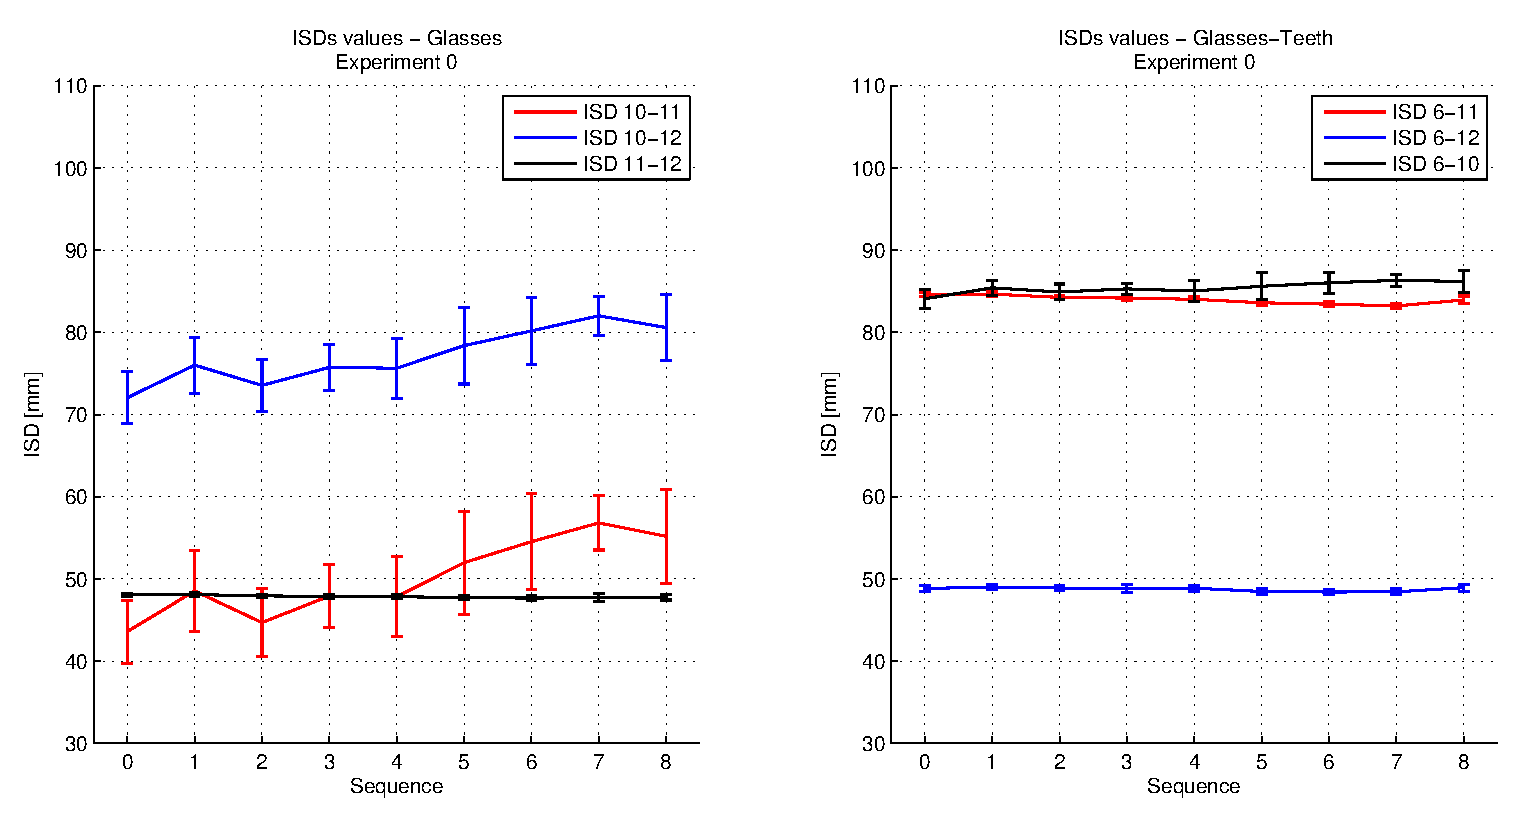
\includegraphics[width=0.75\textwidth]{include/linguometer/images/example_isd_0.eps}}
	\subfigure[\label{fig:linguometer:technical:isd:example:2}]
	{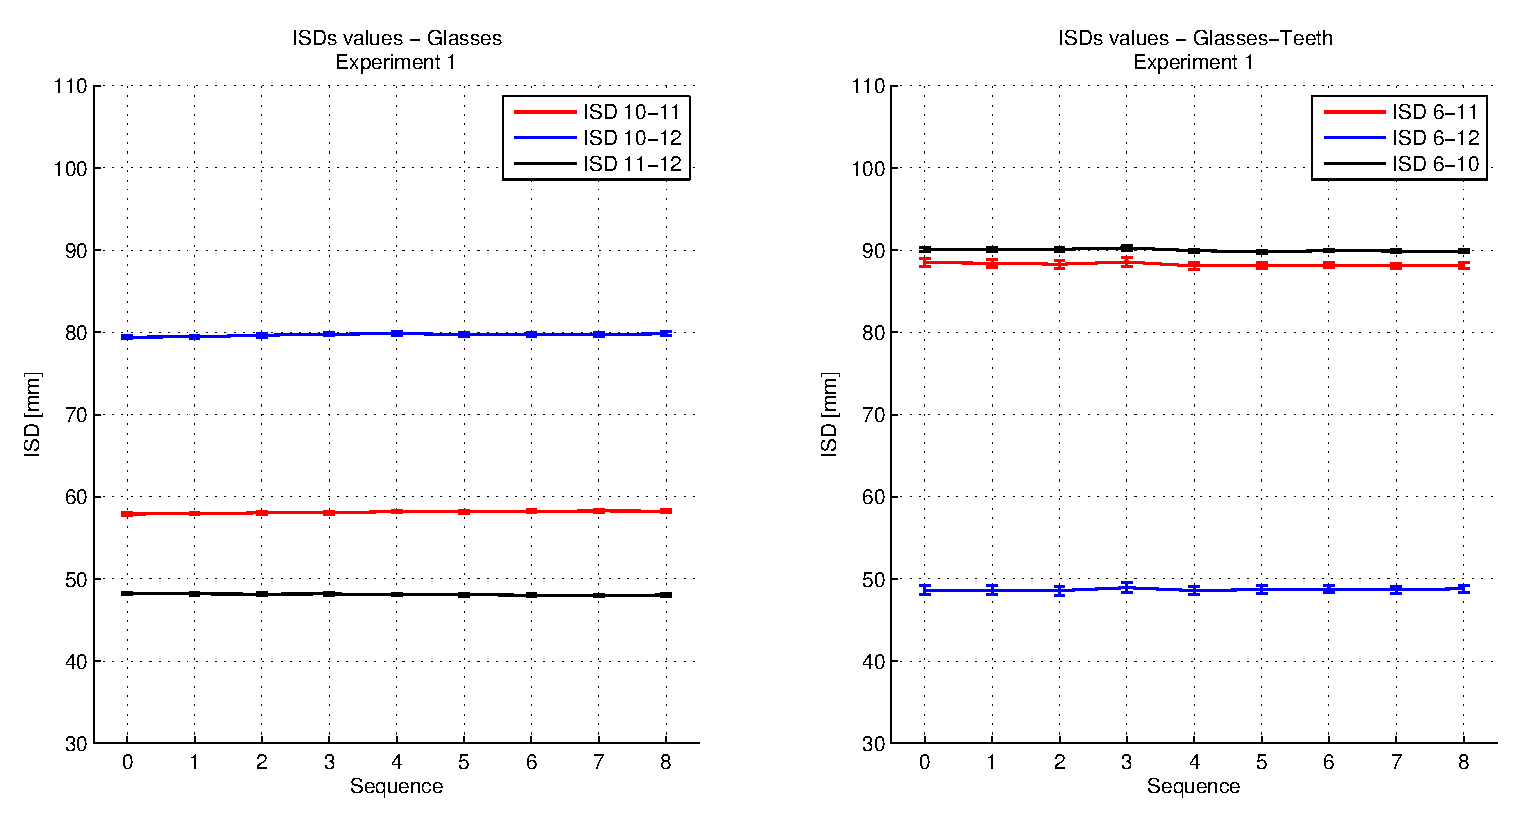
\includegraphics[width=0.75\textwidth]{include/linguometer/images/example_isd_1.eps}}
	\subfigure[\label{fig:linguometer:technical:isd:example:3}]
	{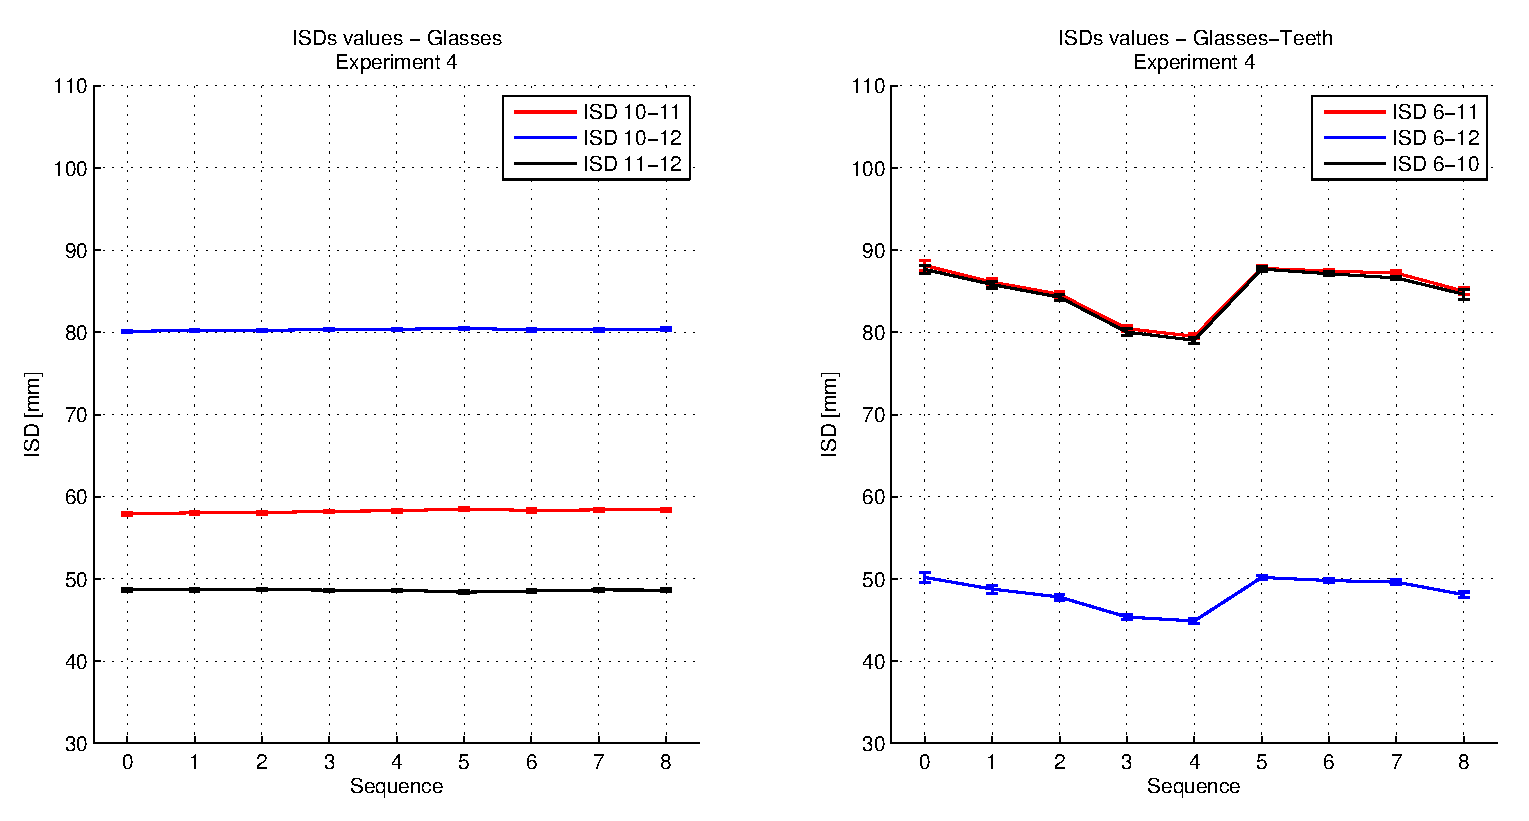
\includegraphics[width=0.75\textwidth]{include/linguometer/images/example_isd_4.eps}}
	\hspace{0.475\textwidth}
	
	\caption[ISD results (experiments)]{\textbf{ISD results
	(experiments)}: verification of
	the quality the kinesthetic data acquired by means of electromagnetic 
	articulography.
	The first plot (a) shows the results of a test experiment, where a sensor
	on the glasses (sensor 10) was left outside the spherical volume.
	}
	\label{fig:linguometer:technical:isd:example}
\end{figure}
% ---------------------------------------------------------------------------- %

Figure~\ref{fig:linguometer:technical:isd:example:2} shows the results of a
perfectly acquired experiment.
The average ISD values remain constant across the nine sequences. Furthermore,
the standard deviation remains low ($<$0.25 mm for couples 10-11, 11-12 and 
10-11) and, more importantly, its module is comparable between different 
sequences (Table~\ref{tab:linguometer:technical:isd:experiments1}).

Also Figure~\ref{fig:linguometer:technical:isd:example:3} shows the 
results of a perfectly acquired experiment, but in this case the reference
glasses kept falling toward the tip of the subject's nose.
This event is clearly highlighted by the profiles of the ISD 6-11 and 6-12
curves.
%The fact that the glasses moved by themselves is described by the
%standard deviation values
%(Table~\ref{tab:linguometer:technical:isd:experiments1}).
Moreover, Figures~\ref{fig:linguometer:technical:glasses:1}
and~\ref{fig:linguometer:technical:glasses:2} show two frames of the video
stream acquired with the camcorder. 
The reader surely noticed the different positions of the glasses in the two
frames. Due to the fact that the glasses are slowly moving toward the tip of 
the nose, the euclidean distance calculated between the 6-11 and
the 6-12 couples decreases, since the reference sensors onto the glasses get 
closer to the reference sensor glued onto the upper teeth.\\

Although the procedure used for data validation it is not based on the direct 
knowledge of the physical properties of the AG500 electromagnetic field, it 
proves to be trustworthy.
%In fact, not only it is possible to verify if the acquired data are somehow
%ruined by the presence of the transducer, but it is also possible to
%discriminate between different physical events (e.g.: sensor too far away from
%the recording volume, glasses sliding towards the tip of the nose).
In first approximation, the electromagnetic field does not seem perturbed 
by an unrecoverable interference, although a more in-depth study is needed.
The author is confident about the provided solution, since it fits 
the experimental protocol requirements (see Section~\ref{ch:experiments}).
% ---------------------------------------------------------------------------- %
%\pagebreak
% ---------------------------------------------------------------------------- %
